\documentclass[a4paper,12pt,twoside]{article}
\usepackage{amsmath}
\usepackage{amssymb}
\usepackage{bm}
\usepackage{booktabs}
\usepackage[small,bf]{caption}
\usepackage{comment}
\usepackage{cuted}
\usepackage[shortlabels]{enumitem}
\usepackage{fancyhdr}
\usepackage{fancybox}
\usepackage{float}
\usepackage[T1]{fontenc}
\usepackage[a4paper,left=1in,right=1in,top=0.25in,bottom=1in,
    headheight=76.33466pt,
    headsep=\dimexpr1in-62.33466pt\relax,
    includehead
]{geometry}
\usepackage{graphicx}
\usepackage{hyperref}
\usepackage[utf8]{inputenc}
% \usepackage{lipsum}
\usepackage{listings}
\usepackage{minted}
\usemintedstyle{emacs}
\usepackage{multirow}
\usepackage{parskip}
\usepackage{ragged2e}
\usepackage{setspace}
\usepackage{soul}
% \onehalfspacing
\usepackage{subcaption}
% \usepackage[subrefformat=parens,labelformat=parens]{subfig}
\usepackage{tabularx}
% \usepackage{titling}
\usepackage{xurl}
\usepackage{biblatex}
\addbibresource{Project.bib}
\usepackage{background}
\backgroundsetup{contents=
\includegraphics{waterprint.jpg}, scale=0.8, opacity=0.1}
\pagestyle{fancy}
\fancyhf{}
\fancyhead[LE,RO]{}
\fancyhead[CE,CO]{
\includegraphics[width=0.7\textwidth]{JILogo.png}}
\fancyhead[RE,LO]{}
\fancyfoot[CE,CO]{\leftmark}
\fancyfoot[CE,CO]{\thepage}
\lfoot{\textit{ECE4810J \textbf{SoC Design} | Fall 2022}}
\renewcommand{\headrulewidth}{1pt}
\renewcommand{\footrulewidth}{1pt}
\definecolor{caption2color}{HTML}{2e5395}
\hypersetup{
    colorlinks=true,
    linkcolor=blue,
    filecolor=magenta,      
    urlcolor=cyan,
    pdfpagemode=FullScreen,
}
\definecolor{codegreen}{rgb}{0,0.6,0}
\definecolor{codegray}{rgb}{0.5,0.5,0.5}
\definecolor{codepurple}{rgb}{0.58,0,0.82}
\definecolor{backcolour}{rgb}{0.95,0.95,0.92}
\newcommand{\code}[1]{\texttt{#1}}

\lstdefinestyle{mystyle}{
    backgroundcolor=\color{backcolour},   
    commentstyle=\color{codegreen},
    keywordstyle=\color{magenta},
    numberstyle=\tiny\color{codegray},
    stringstyle=\color{codepurple},
    basicstyle=\ttfamily\footnotesize,
    breakatwhitespace=false,         
    breaklines=true,                 
    captionpos=b,                    
    keepspaces=true,                 
    numbers=left,                    
    numbersep=5pt,                  
    showspaces=false,                
    showstringspaces=false,
    showtabs=false,                  
    tabsize=2
}

\lstset{style=mystyle}

\author{Xinfei Guo, Yihua Liu}
\title{ECE4810J FA2022\\ \small Final Project}
\date{November 14, 2022}

\begin{document}
% \maketitle
\thispagestyle{fancy}

\begin{center}
    \vspace*{0pt}
    \Large{\textbf{ECE4810J SoC Design}}\\
    \vspace*{2pt}
    \large{Fall 2022}\\
    \vspace*{10pt}
    \Large{\textcolor{caption2color}{Final Project}}\\
%    \normalsize{\hl{Due: 11:59pm Oct. 23rd, 2022}}
    \rule[-5pt]{.97\linewidth}{0.05em}
\end{center}

\textbf{Logistics:}
\begin{itemize}
    \item This project is a team exercise.
    \item Please use the discussion board on Piazza for Q\&A.
    \item All reports and code (if available) MUST be submitted to the assignment of Canvas.
    \item Internet usage is allowed and encouraged.
    \item The deadlines are final, no late submission is allowed for this project.
    \item Creativity is highly encouraged and will be credited for this project.
\end{itemize}
\newpage
\tableofcontents
\newpage
\section{Project Description}
In this class, we have learned various SoC design methodologies (FPGA \& ASIC) together with different flavors of design languages (Verilog, HLS, Python, etc.). We also covered different components of an SoC (processor, interconnect, interface, etc.) and design tradeoffs. In this final project, you will have opportunities to try out one or more of these design approaches/languages and experience an actual design process from concept to implementation. \textbf{This is a team-based project, you will work in the same team (2 or 3 students) as in the lab sessions}. 

The goal of this project is to offer you practical experiences of designing a relatively large-scale chip and explore the design tradeoffs by employing the design flows (listed below) learned in the labs. Based on interests, each team will pick one unique topic from the pool in Section \ref{topicpool}, and the selection process will be announced separately.

Flow Options:
\begin{itemize}
    \item FPGA flow with Verilog/SystemVerilog/SystemC + board evaluation on Arty Z7 by Vitis or Pynq\footnote{The board evaluation by Pynq see Lab 3 Section 6.}
    \item FPGA flow with Vitis HLS + board evaluation on Arty Z7 by Vitis or Pynq\footnote{For Vitis HLS, you have to apply the optimization methods to optimize your HLS design and show how your design is optimized.}
    \item FPGA flow with MATLAB HDL Coder + Simulink + board evaluation on Arty Z7 by Vitis or Pynq\footnote{If applicable, you can also use Xilinx System Generator (SysGen).}
    \item PYNQ flow with Python + board evaluation on Arty Z7
    \item ASIC flow with OpenRoad tool suite (SkyWater 130nm)
    \item ASIC flow with Synopsys tool suite (Synopsys 32/28nm or 90nm or FreePDK 45nm)\footnote{The full ASIC flow using FreePDK 45nm see Lab 6 Section 3 \& 4.}
    \item Design with high-level languages such as PyMTL
\end{itemize}
\begin{figure}[H]
    \centering
    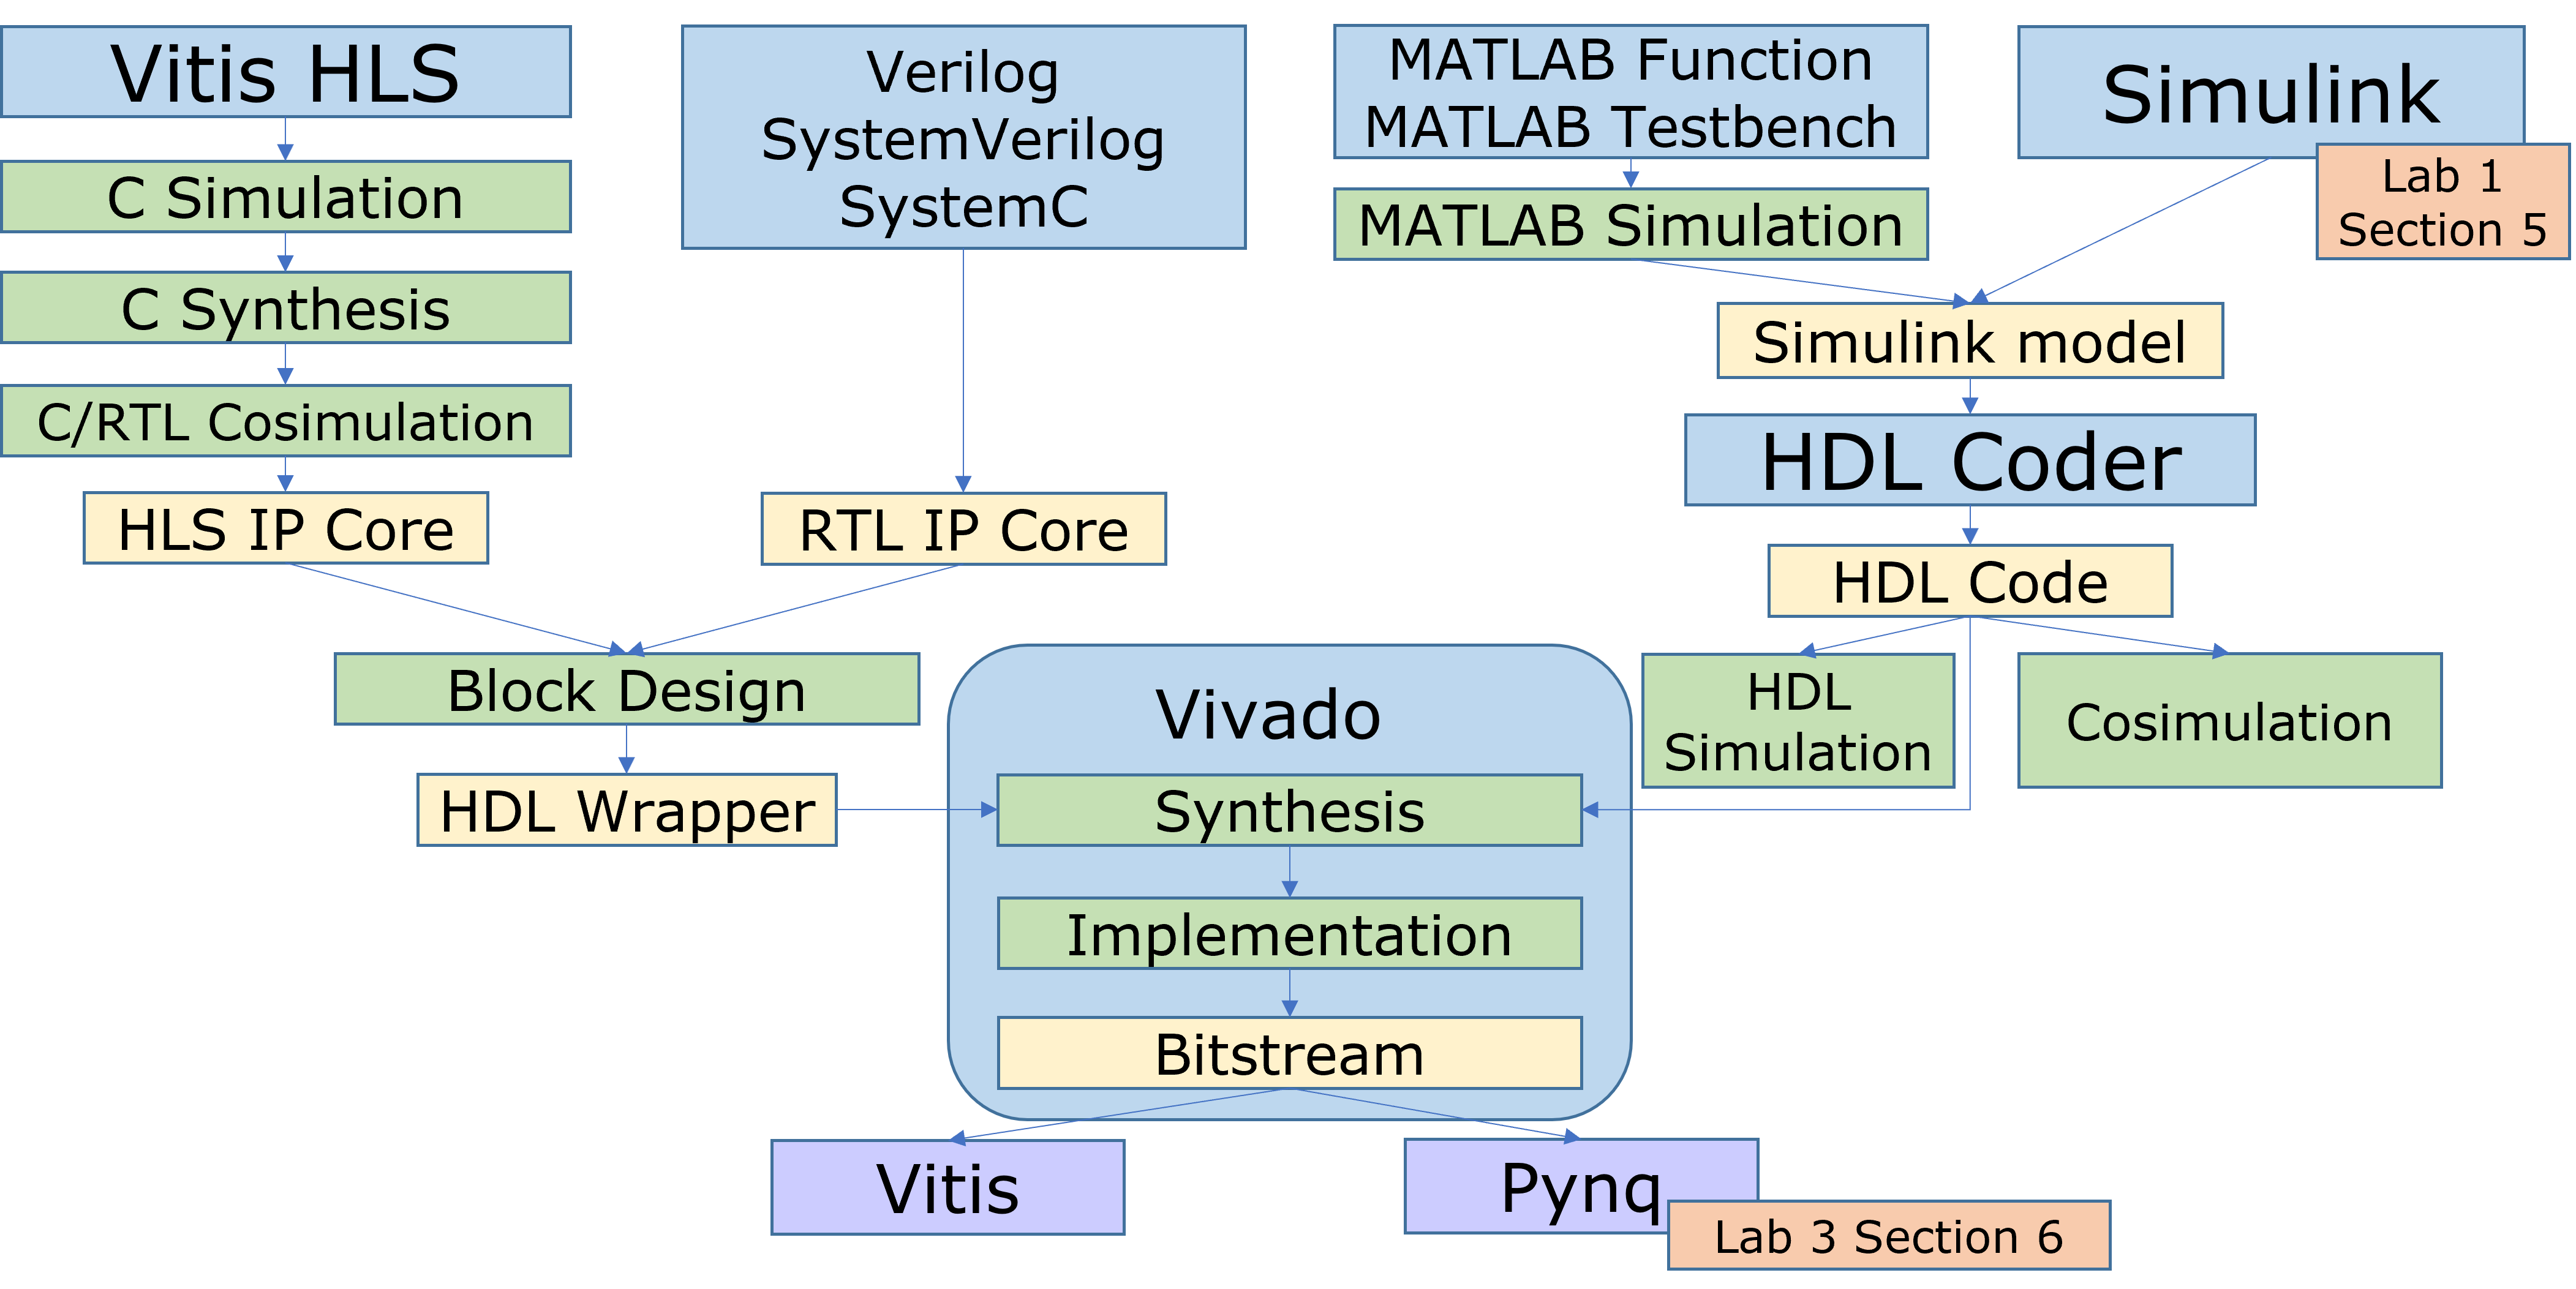
\includegraphics[width=\textwidth]{images/23.png}
\end{figure}
\begin{figure}[H]
    \centering
    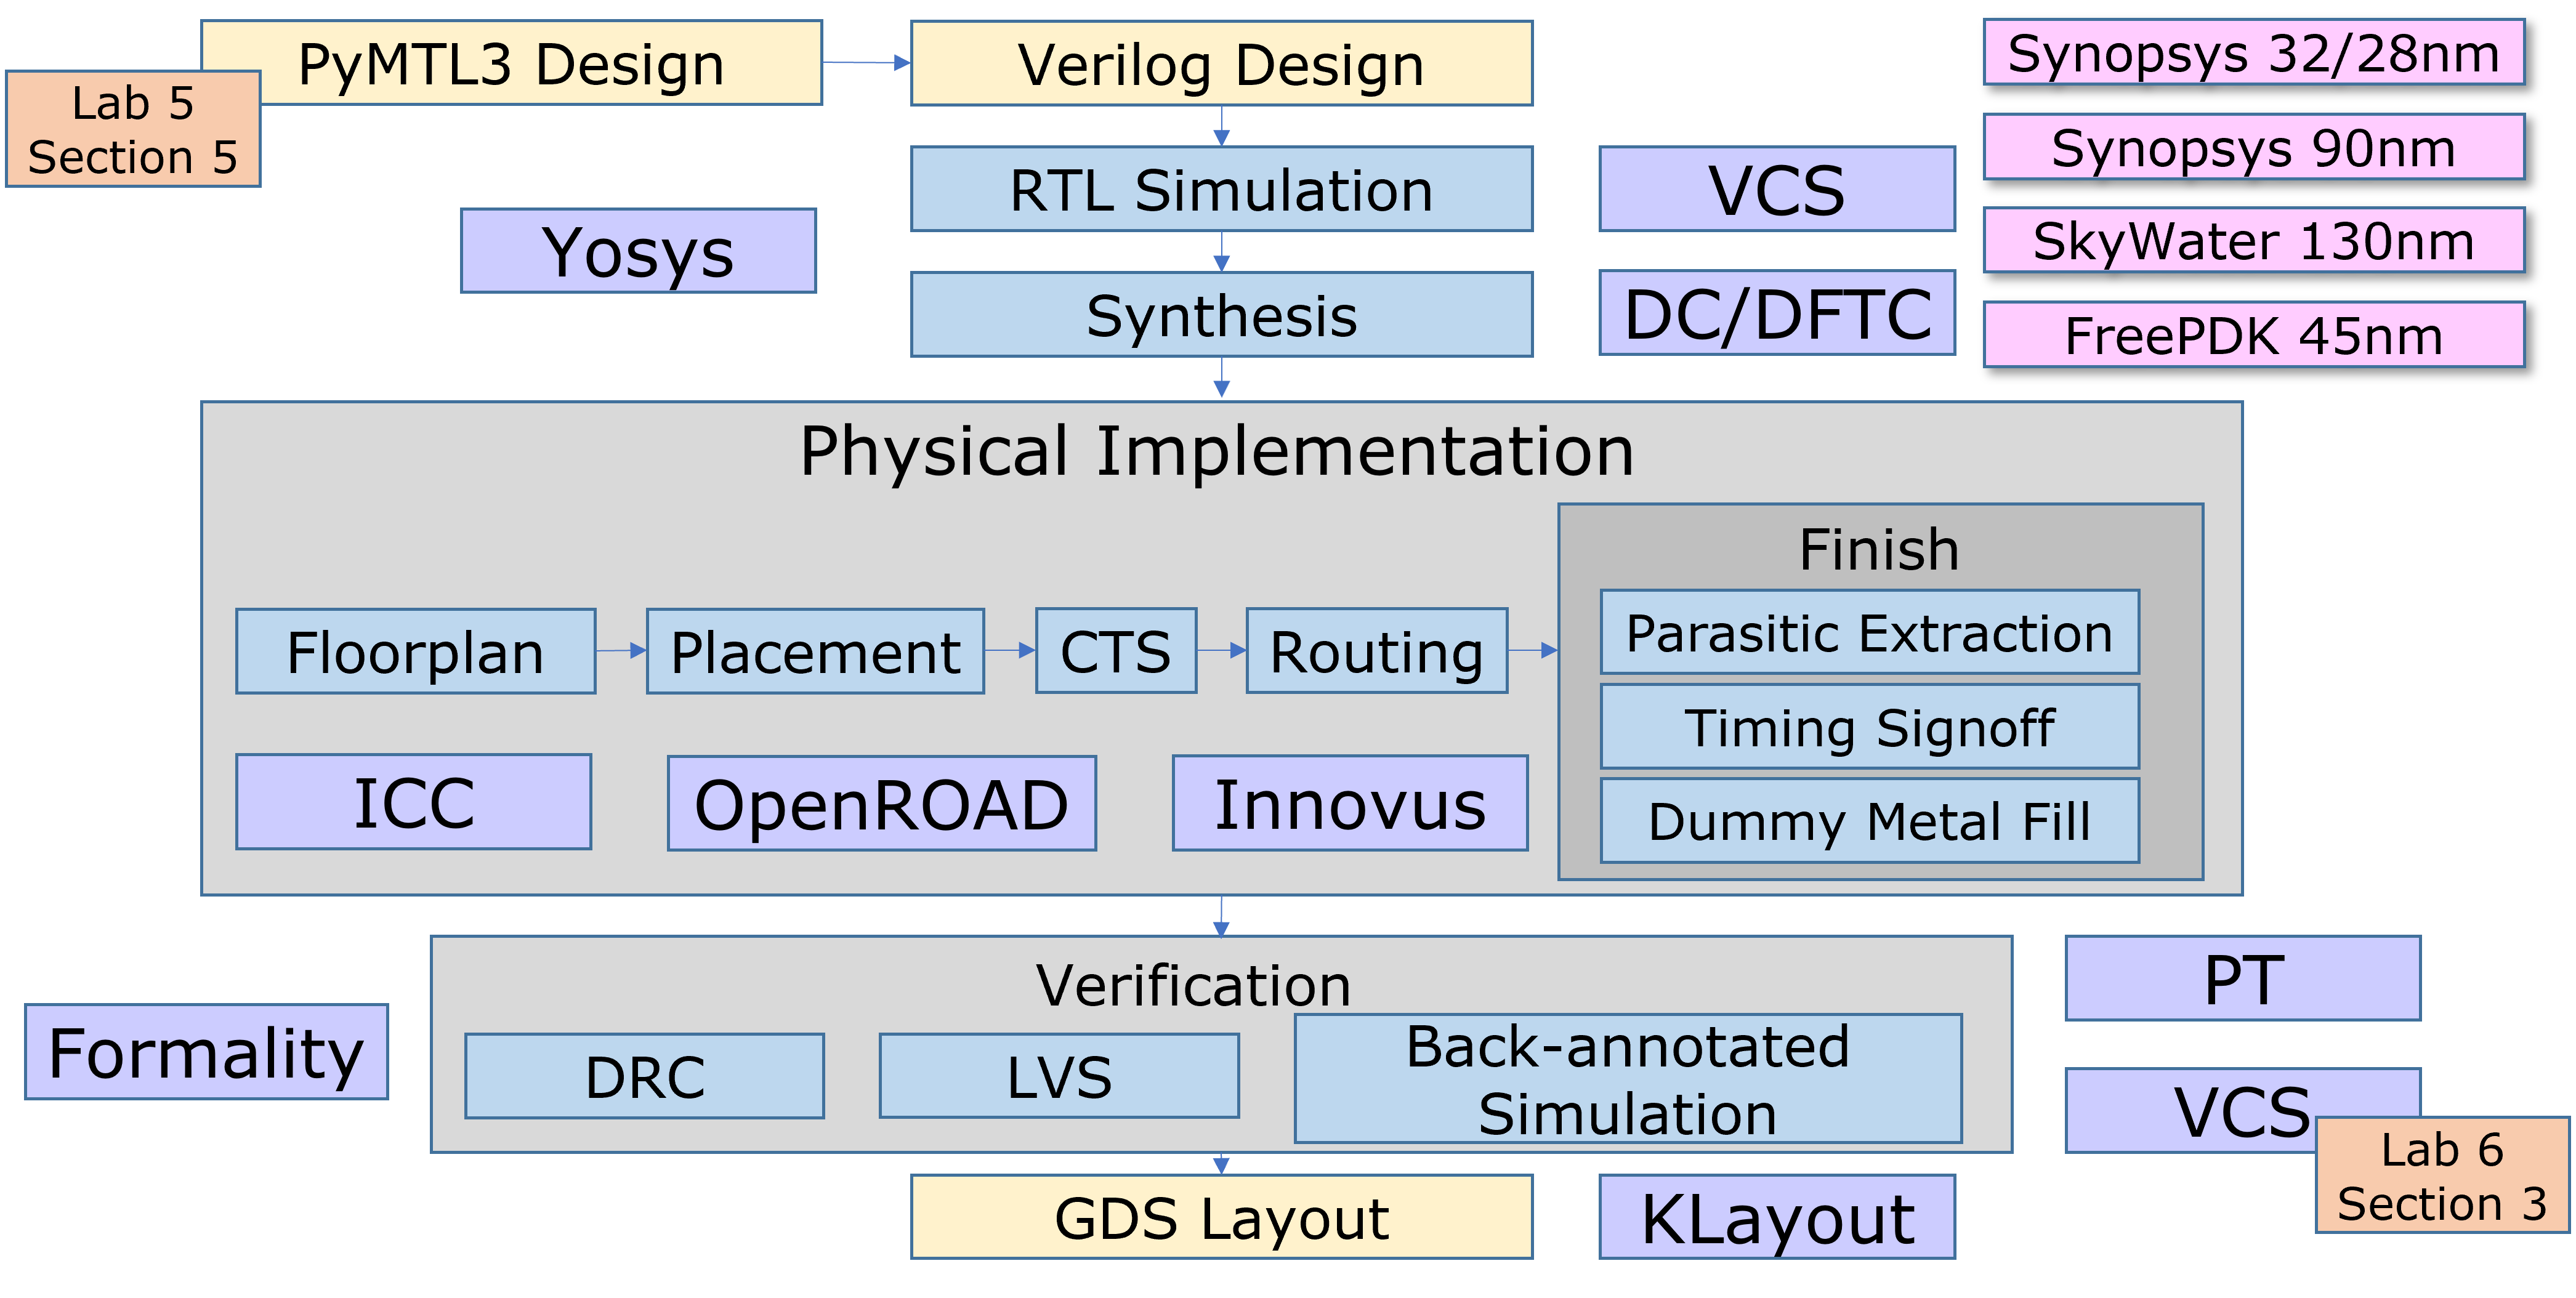
\includegraphics[width=\textwidth]{images/24.png}
\end{figure}

\section{Project Topic Pool (not in particular order)} 
\label{topicpool}
\subsection{Physical Implementation with FPGA and ASIC Flows}
In this project, you are given the following designs, and you need to implement them with FPGA and ASIC flows, respectively. For ASIC flow, you can choose Synopsys or Open-source tools, and you can also choose any PDK and cell library you like. You are responsible for writing all constraints (SDC, Tcl, etc.), and you are also required to explain how you choose the parameters for major physical design implementation steps. 

Design I: APU block from \url{https://github.com/The-OpenROAD-Project/OpenLane/blob/master/designs/APU/src/APU.v}

Design II: usb2p0 block from \url{https://github.com/The-OpenROAD-Project/OpenLane/blob/master/designs/usb/src/usb2p0_core.v}

During your implementation, please address the following aspects.
\begin{itemize}
    \item Please define a way to make a ``fair'' comparison among the ASIC and FPGA flows. The metrics to compare include but are not limited to power, performance, and area. The key is to dive into the reason why the two implementation flows give very different results. You need to explain it or prove your hypothesis by conducting experiments instead of using plain words.
    \item In ASIC implementation, please describe your floorplanning strategy in terms of how you pick the aspect ratio, how you place pins, how you develop your power grid and what the reasons are.
    \item In both FPGA and ASIC flows, please decide the maximum frequency for the design and analyze the critical paths.
    \item In both FPGA and ASIC flows, please pick top-5 timing critical paths after place and route and analyze them by giving the reason why they are slower than other paths (e.g., they have too many levels of logic, the cells are also based on regular Vth instead of low Vth). Propose at least one solution to speed up the path.
    \item Please explain any challenges you face in implementing these designs with either FPGA or ASIC flows.    
\end{itemize}

\subsection{Design-space exploration with OpenLane Design Flow}
This project starts from Lab 4 Section 6.

OpenLane comes with a convenient mechanism for running flows with a range of \href{https://github.com/efabless/openlane#adding-a-design}{configuration options}. In this project, you will first implement the following APU and usb2p0 designs with the OpenLane flow using the flow default parameters. You will then need to define a ``regression'' configuration file in \code{\$\{OPENLANE\_ROOT\}/designs/apu/regression.config}. An example is shown below.

\begin{verbatim}
CLOCK_PERIOD=(1 2 5 10)
GLB_RT_ADJUSTMENT=(0 0.15)
FP_CORE_UTIL=(10 25 50)
PL_TARGET_DENSITY=(0.05 0.1 0.2)
SYNTH_STRATEGY=(1 3 14)

extra="
"
\end{verbatim}

There is some documentation for these parameters \href{https://github.com/efabless/openlane/blob/master/configuration/README.md}{here}. See also \href{https://github.com/efabless/openlane/wiki#what-is-the-difference-between-fp_core_util-and-pl_target_density}{this explanation} of \code{FP\_CORE\_UTIL} vs \code{PL\_TARGET\_DENSITY}.

Design I: APU block from \url{https://github.com/The-OpenROAD-Project/OpenLane/blob/master/designs/APU/src/APU.v}

Design II: usb2p0 block from \url{https://github.com/The-OpenROAD-Project/OpenLane/blob/master/designs/usb/src/usb2p0_core.v}

Set up the regression config and run the regresion tool to look at the following aspects for the design, for example, if you are looking for the tightest clock timing for the design. You can do
\begin{verbatim}
cd ${OPENLANE_ROOT}
docker run -it -v $(pwd):/openLANE_flow -v \\
$PDK_ROOT:$PDK_ROOT -e PDK_ROOT=$PDK_ROOT \\
-u $(id -u $USER):$(id -g $USER) openlane:rc2
# in the container:
python3 run_designs.py --designs gcd \\
--regression designs/gcd/regression.config --threads 4
\end{verbatim}

The aspects to look at for this project include: 
\begin{itemize}
    \item Run the regression test to check the maximum core utilization for your design.
    \item Turn on the placement timing driven and compare against a base case, any changes in timing? Please describe the timing differences.
    \item Try to run synthesis at a different corner (by changing LIB\_SYNTH to a use the same lib defined by LIB\_SLOWEST. Please find out the maximum clock cycle for the design. How will area and power chance under this new corner?
    \item Sweep the target skew for clock tree synthesis and observe the differences. Explain the differences.
    \item Change the core utilization to 2:1, 3:1 and 4:1, what did you observe? Any changes about timing, area and power? Why did this change happen. Please upload the screenshot of the layout after changing the aspect ratio.
    \item Pick two parameters (from \href{https://github.com/efabless/openlane/blob/master/configuration/README.md}{here}) for placement and routing respectively, conduct a fine-grain sweep of the parameter vs. PPA, and explain your observations. 
    \item In general, please explain the design space exploration process and all the challenges you have faced during the process. It would be good if you can please provide several potential solutions to overcome these challenges.   
\end{itemize}

\subsection{Matrix Multiplication Accelerator}
Matrix multiplication is a traditionally intense mathematical operation for most processors. Despite having applications in computer graphics and high-performance physics simulations, matrix multiplication operations are still relatively slow on general purpose hardware, and require significant resource investment (high memory allocations, plus at least one multiply and add per cell). We set out to design an accelerator to not only speed up the operations, but also allow offloading of the execution to free up general processor time for other tasks. As an added bonus, accelerators, because they don't contain any processing elements that aren't necessary, typically are more efficient at the task at hand, requiring less power to run than a general-purpose implementation.

For the register-based approach, we wanted to create a design that would be able to perform matrix multiplications in as few cycles as possible. To this extent, we realized that each value in the output matrix could be calculated completely independently, since each value in the output matrix only depends on one row in m1 being multiplied with one column of m2. To take advantage of this massive parallelism, we needed to store our matrices in a data structure that allowed us to write many values into the output matrix simultaneously, and we needed to be able to read many different values from our input matrices simultaneously. This was the reason we decided to implement this data structure from registers. The overall design can be seen below in Figure \ref{mac_2x2}.
\begin{figure}[H]
    \centering
    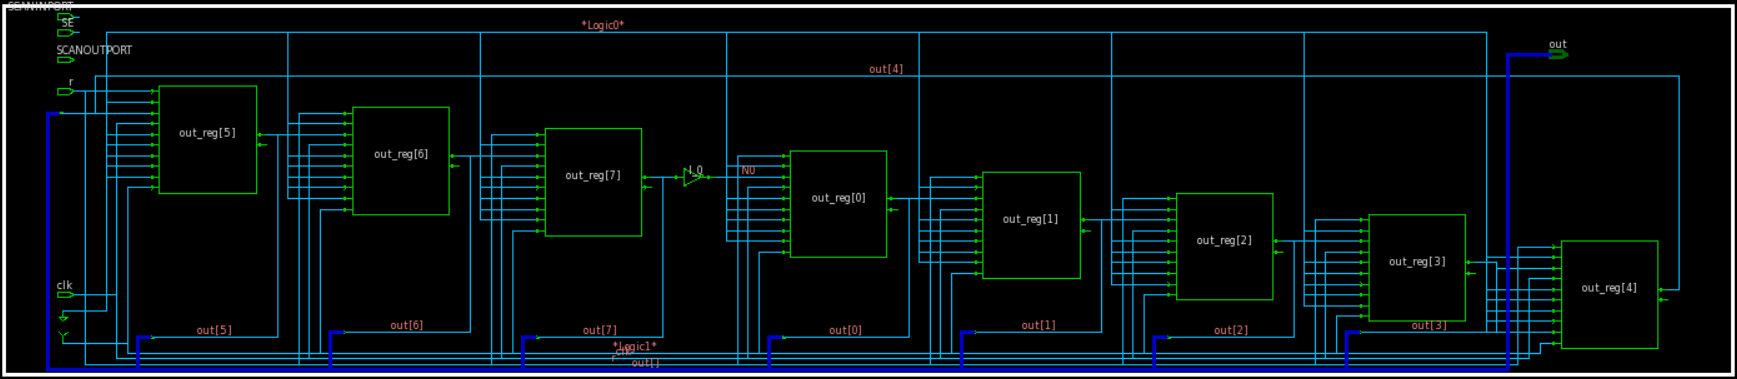
\includegraphics[width=0.6\textwidth]{images/25.jpg}
    \caption{2x2 Example of Register-Based Design.}
    \label{mac_2x2}
\end{figure}
We hoped to achieve better `single threaded' performance by increasing the clock frequency and pipelining the multiply-accumulations as much as possible with this scenario.
We compare both of these solutions to a simple implementation of matrix multiplication written in C. This is a straightforward O(n3) implementation that essentially performs the same operations as the hardware does, which can be seen in Listing \ref{MM_ccode}. This gave us an interesting comparison because while the ARM Hard Processor System (HPS) is running at almost 10x the clock frequency of the hardware we designed, there is far more overhead for any given instruction running in C than in the hardware. For example, in the C code, there are branches for the for loops that must be predicted and resolved, there are cache misses that would require far more cycles to retrieve a value from main memory, and loads and stores cannot happen simultaneously to each of the matrices. So, if our hardware were to keep up with the HPS, it would have to be far more efficient, taking full advantage of each cycle.
\begin{listing}[H]
\begin{minted}{c}
for (i = 0; i < MATRIX_SIZE; i++) {
    for (j = 0; j < MATRIX_SIZE; j++) {
        accum = 0;
        for (k = 0; k < MATRIX_SIZE; k++) {
            accum += (m1[k][j] * m2[i][k]);
        }
        res[i][j] = accum;
    }
}
\end{minted}
\caption{C Code Implementation of Matrix Multiply.}
\label{MM_ccode}
\end{listing}
In this project, you are expected to come up with novel ways to accelerate matrix multiplication with hardware approaches.

\textbf{References}
\begin{itemize}
    \item \url{http://csg.csail.mit.edu/pubs/bluespec/HardwareAcceleration.pdf}
    \item \url{http://www.diva-portal.org/smash/get/diva2:1265778/FULLTEXT01.pdf}
    \item \url{http://citeseerx.ist.psu.edu/viewdoc/download?doi=10.1.1.301.3662&rep=rep1&type=pdf}

\end{itemize}

\subsection{Wishbone Bus Implementation}
The WISHBONE System-On-Chip (SOC) Interconnection Architecture, also known as WISHBONE Bus, is a free, open-source standard that defines a common interface among IP Cores in a System-On-Chip. By doing so, it alleviates integration problems. That, in turn, encourages IP reuse which leads to improvements in the portability and reliability of the system and results in faster time-to-market for the end users.

WISHBONE is intended as a general-purpose portable interface that is independent of the underlying semiconductor technology. As such, its specification defines a set of signals and bus cycles but does not specify any electrical information nor enforce a bus topology. The WISHBONE bus uses a MASTER/SLAVE model of communication. In this model, the MASTER entities are capable of driving the bus by generating bus cycles, whereas SLAVES entities may only use the bus when instructed/inquired by a MASTER.

\textbf{Wishbone Interconnection (INTERCON)}\\
The interconnection is the component responsible for tying all the various subcomponents/entities, MASTERS and SLAVES, together in a manner that meets all communication and timing needs. Implementation requirements:
\begin{itemize}
    \item Uses a shared bus topology: Care must be taken so that just one participant drives the bus at any time.
    \item Based on multiplexers: One other tricky part of designing a shared bus inside an FPGA is that bus participants who are not driving the bus must neither drive a low nor a high signal on the bus. Typically, this is achieved by setting the signal drivers to a ``High-Z'' state, which means using Tri-State buffers. Since, normally, FPGAs do not have internal Tri-States buffers a switch logic based on multiplexers was implemented.
    \item 1 to N multiplexing (1 Masters, N Slaves): The facts that this is a single MASTER implementation and SLAVES may not use the bus when not addressed, the only care that must be taken is to not overlap the SLAVES memory maps.
    \item Partial address decoding: Each slave present in the bus has a corresponding entry in the memory map. Each of these entries consists of a base address (BASEADDR) and a size (SIZE). The SIZE corresponds to the effective number of addresses occupied by the slave, starting at the BASEADDR. In other words, this SIZE corresponds to the maximum OFFSET.
\end{itemize}

The decoding process is done in two steps: The first step is done by comparators (one for each slave) implemented in this interconnection block. These comparators use the base address to select the slave or not. They do this by masking out the OFFSET bits of the address and then comparing base addresses. The masking out of the OFFSET bits is achieved using the SIZE. The second step is done by a fine decoder inside the selected slave. It will receive just the OFFSET and verify if it is valid.

Using this decoding scheme has the drawback of imposing that the number of addresses used by the slaves must be a power of two, even when not all addresses are used. Hence, memory addresses can be wasted.

\textbf{References:}
\begin{itemize}
    \item \url{https://arxiv.org/ftp/arxiv/papers/1205/1205.1860.pdf}
    \item \url{https://github.com/boschmitt/wishbone}
    \item \url{https://opencores.org/howto/wishbone}
\end{itemize}

\subsection{JPEG Encoder \& Decoder}
\subsubsection{Tasks}
The algorithms of JPEG encoding and decoding are introduced in Lab 3 Section 4. For this project, you can reuse the YUV model and DCT you implement in Lab 3 and mainly implement a Huffman encoder \& decoder. However, your algorithm should follow the mainstream standard JPEG implementation like \href{https://github.com/LuaDist/libjpeg}{libjpeg} and \href{https://github.com/libjpeg-turbo/libjpeg-turbo}{libjpeg-turbo} as mentioned in Lab 3, for example, you should use the Butterfly algorithm to optimize your DCT design. The choice of the quantization matrix is up to you as long as it produces nice images. Your testbenches have to be real JPG pictures such as Lenna or its alternatives \cite{doi:10.1080/09500340.2016.1270881}. The decoded data of your encoded data have to be similar to your original data.
\subsubsection{Huffman Coding}
For Huffman coding, you should consider using Canonical Huffman coding instead of traditional Huffman coding. Canonical Huffman coding has two main benefits over traditional Huffman coding. In basic Huffman coding, the encoder passes the complete Huffman tree structure to the decoder. Therefore, the decoder must traverse the tree to decode every encoded symbol. On the other hand, canonical Huffman coding only transfers the number of bits for each symbol to the decoder, and the decoder reconstructs the codeword for each symbol. This makes the decoder more efficient both in memory usage, and computation requirements \cite{2018arXiv180503648K}.

In basic Huffman coding, the decoder decompresses the data by traversing the Huffman tree from the root until it hits the leaf node. This has two major drawbacks: it requires storing the entire Huffman tree, which increases memory usage. Furthermore, traversing the tree for each symbol is computationally expensive. Canonical Huffman encoding addresses these two issues by creating codes using a standardized canonical format. The benefit of using canonical encoding is that we only need to transmit the length of each Huffman codeword. A Canonical Huffman code has two additional properties. Firstly, longer-length codes have a higher numeric value than the same-length prefix of shorter codes. Secondly, codes with the same length increase by one as the symbol value increases. This means if we know the starting symbol for each code length, we can easily reconstruct the canonical Huffman code. The Huffman tree is essentially equivalent to a ‘sorted’ version of the original Huffman tree so that longer codewords are on the right-most branch of the tree and all of the nodes at the same level of the tree are sorted in order of the symbols.
\begin{figure}[H]
    \centering
    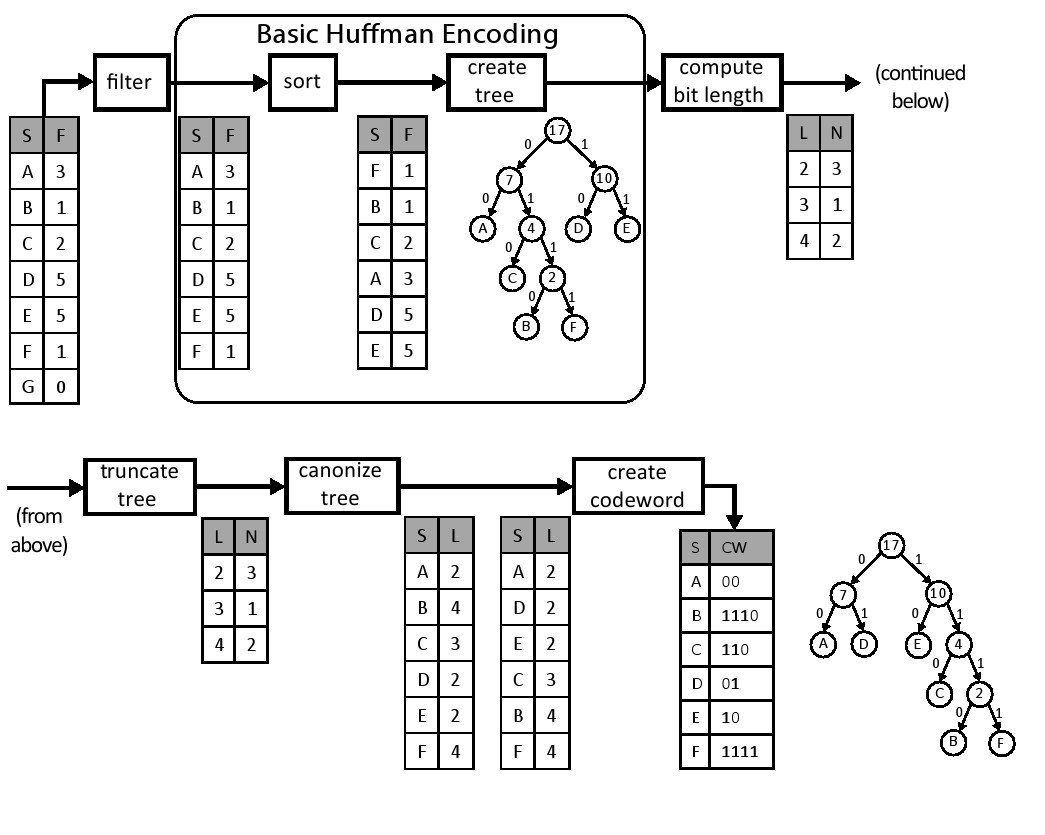
\includegraphics[width=0.8\textwidth]{images/1.jpg}
    \caption{The Canonical Huffman Encoding process. The symbols are filtered and sorted and used to build a Huffman tree. Instead of passing the entire tree to the decoder (as is done in “basic” Huffman coding), the encoding is done such that only the length of the symbols in the tree is required by the decoder. Note that the final canonical tree is different from the initial tree created near the beginning of the process.}
\end{figure}
\begin{figure}[H]
    \centering
    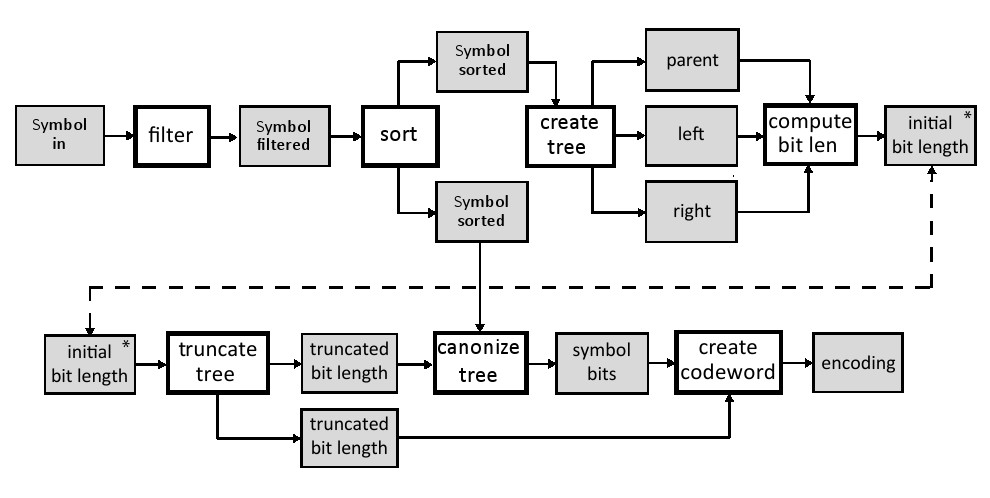
\includegraphics[width=\textwidth]{images/2.jpg}
    \caption{The block diagram for the sample hardware implementation of canonical Huffman encoding. The gray blocks represent the significant input and output data that is generated and consumed by the different subfunctions. The white blocks correspond to the functions (computational cores). Note that the array's initial bit length appears twice to allow the figure to be more clear.}
\end{figure}

\subsection{CORDIC and Phase Detector}
\subsubsection{Introduction}
In this project, you are firstly required to implement a Cartesian to Polar transform in two different ways: using CORDIC and as a lookup table (LUT). Then, you are required to design a simple phase detector. This is done by combining a complex FIR filter and a COordinate Rotation DIgital Computer (CORDIC). You build a complex FIR filter by hierarchically instantiating four “real” FIR filters similar to what you developed in Lab 3 Section 6.

The complex FIR filter is used to correlate to a known complex signal. We use Golay codes which have some great properties related to orthogonality and auto-correlation. This is not important to this project but it is some really amazing math. We hope you look into it.

In the end, you will combine all of these modules into a phase detector. This is a common block used in a digital communications receiver. The goal is to do simple synchronization and discover the phase of the signal. The output of the CORDIC (r, theta) gives you these results. It is a simple phase detector but should provide you with a basic understanding of the problem, and you should come away with knowledge on how to develop two new important hardware blocks (CORDIC and a complex FIR filter).

We provide a Simulink file that models a transmitter, channel, and receiver. You are building an equivalent receiver in HLS in this project. The Simulink file is provided for your information only. You do not have to edit or do anything with this file though it could be useful for understanding the overall application better.
\subsubsection{CORDIC IP}
In Lab 2, we have an IP core that can do all the RV32IM operations. However, how to do more complex calculations like trigonometric, logarithmic, exponential, and power functions? The answer is CORDIC.

CORDIC is an efficient technique for calculating trigonometric, hyperbolic, and other mathematical functions. It is a digit-by-digit algorithm that produces one output digit per iteration. This allows us to tune the accuracy of the algorithm to the application requirements; additional iterations produce a more precise output result. Accuracy is another common design evaluation metric alongside performance and resource usage. CORDIC performs simple computations using only addition, subtraction, bit shifting, and table lookups, which are efficient to implement in FPGAs and, more generally, in hardware.
\begin{figure}[H]
    \centering
    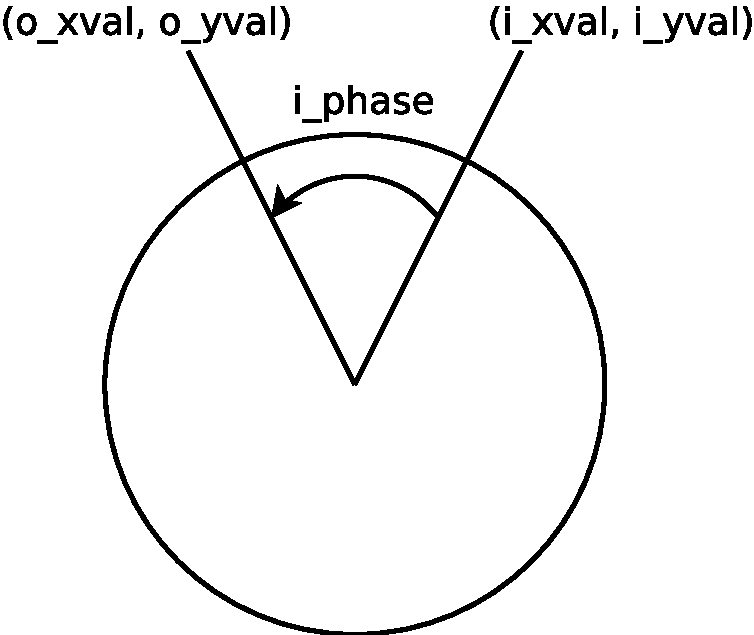
\includegraphics[width=0.5\textwidth]{images/3.pdf}
    \caption{The CORDIC problem description.}
\end{figure}
The CORDIC method was developed by Jack Volder in the 1950s as a digital solution to replace an analog resolver for real-time navigation on a B-58 bomber. A resolver measures degrees of rotation. At that time, hardware implementations of multiplication operations were prohibitively expensive, and CPUs had a very limited amount of state. Thus the algorithm needed to have low complexity and use simple operations. Over the years, it has been used in math
co-processors, linear systems, radar signal processing, Fourier transforms, and many other digital signal processing algorithms. It is now commonly used in FPGA designs. Vitis HLS uses a CORDIC core for calculating trigonometric functions, and it is a common element of modern FPGA IP core libraries.

A simple two-dimensional rotation matrix is given by:
\begin{equation}
    R(\theta)=\begin{pmatrix}
        \cos{(\theta)}&-\sin{(\theta)}\\
        \sin{(\theta)}&\cos{(\theta)}
    \end{pmatrix}
\end{equation}
This rotation can be used to rotate a complex vector $\exp{(j*\phi)}$ and turn it into another one, $\exp{(j*(\phi+\theta))}$ if the real value is the first value in the given vector, and the would-be imaginary value the second (i.e., strip off the $j$). Further, if the original vector is simply the real number one, $1+j0$, then we will have just created $\sin{\theta}$ and $\cos{\theta}$ in this process.

The CORDIC approach is to replace the cosine portion of this rotation matrix with a 1 and the sine portion with a $2^{-k}$.
\begin{equation}
    T(2^{-k})=\begin{pmatrix}
        1&-2^{-k}\\
        2^{-k}&1
    \end{pmatrix}
\end{equation}
You can think of this as a series of complex rotation vectors indexed by $k$, such as those shown in Fig 1. Notice from the figure that these vectors are not on the unit circle but rather just outside the unit circle, and they get closer and closer to the unit circle the higher $k$ becomes.
\begin{figure}[H]
    \centering
    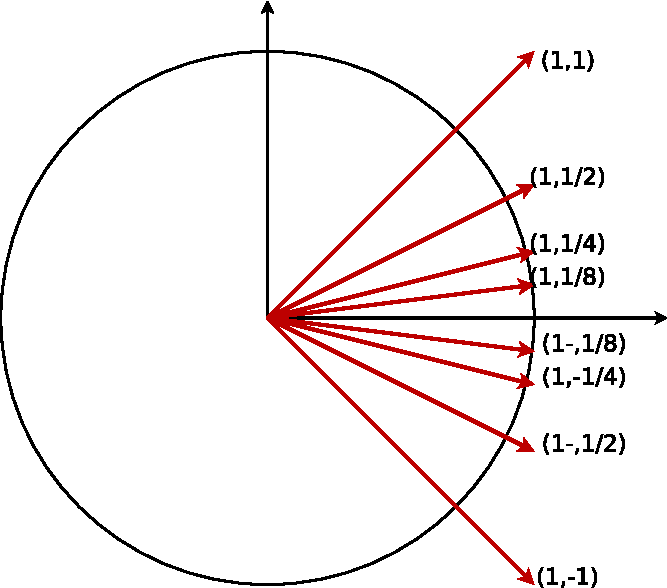
\includegraphics[width=0.5\textwidth]{images/4.pdf}
    \caption{CORDIC Rotation Vectors.}
\end{figure}
In other words, $T$ is approximately a rotation matrix.

$T$ is also something that is easy to calculate within an FPGA. It requires only adds, subtracts, and shifts.
\begin{equation}
\begin{array}{cccc}
    x_{k+1}=&x_k&-&(y_k>>k)\\
    y_{k+1}=&(x_k>>k)&+&y_k
\end{array}
\end{equation}
This can all be done with simple integer math–no multiplications or divisions are required. Of course, this transform is not a true rotation matrix. Instead, it is a scaled rotation matrix.

The CORDIC can compute the following functions:
\begin{equation}
\begin{array}{cc}
    \sin{z} & \cos{z} \\
    \arctan{z} & \sinh{z} \\
    \cosh{z} & \tanh^{-1}{z} \\
    \frac{y}{x} & xz \\
    \arctan{\frac{y}{x}} & \sqrt{x^2+y^2} \\
    \sqrt{x^2-y^2} & e^z=\sinh{z}+\cosh{z}
\end{array}
\end{equation}
and indirectly derive the following functions:
\begin{equation}
\begin{array}{cc}
    \tan{z}=\frac{\sin{z}}{\cos{z}} & \arccos{w}=\arctan{\frac{\sqrt{1-w^2}}{w}} \\
    \tanh{z}=\frac{\sinh{z}}{\cosh{z}} & \arcsin{w}=\arctan{\frac{\sqrt{w}}{1-w^2}} \\
    \ln{w}=2\tanh^{-1}{\frac{w-1}{w+1}} & \log_bw=\frac{\ln{w}}{\ln{b}} \\
    w^t=e^{t\ln{w}} & \cosh^{-1}=\ln{(w+\sqrt{1-w^2})} \\
    \arctan{\frac{y}{x}} & \sinh^{-1}=\ln{(w+\sqrt{1+w^2})} \\
    \sqrt{x^2-y^2} & \sqrt{w}=\sqrt{(w+\frac{1}{4})^2-(w-\frac{1}{4})^2}
\end{array}
\end{equation}
You are required to test all these operations on your testbenches.

The iterative bit-parallel implementation of CORDIC is
\begin{figure}[H]
    \centering
    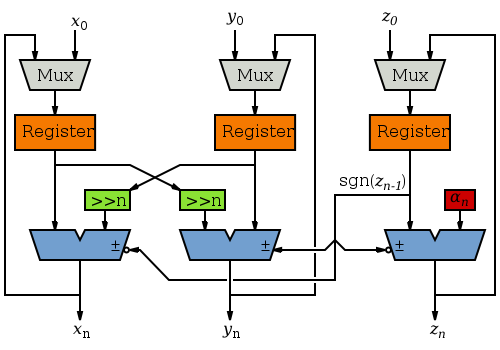
\includegraphics[width=0.7\textwidth]{images/5.png}
\end{figure}
You should consider the unrolled bit-parallel implementation of CORDIC
\begin{figure}[H]
    \centering
    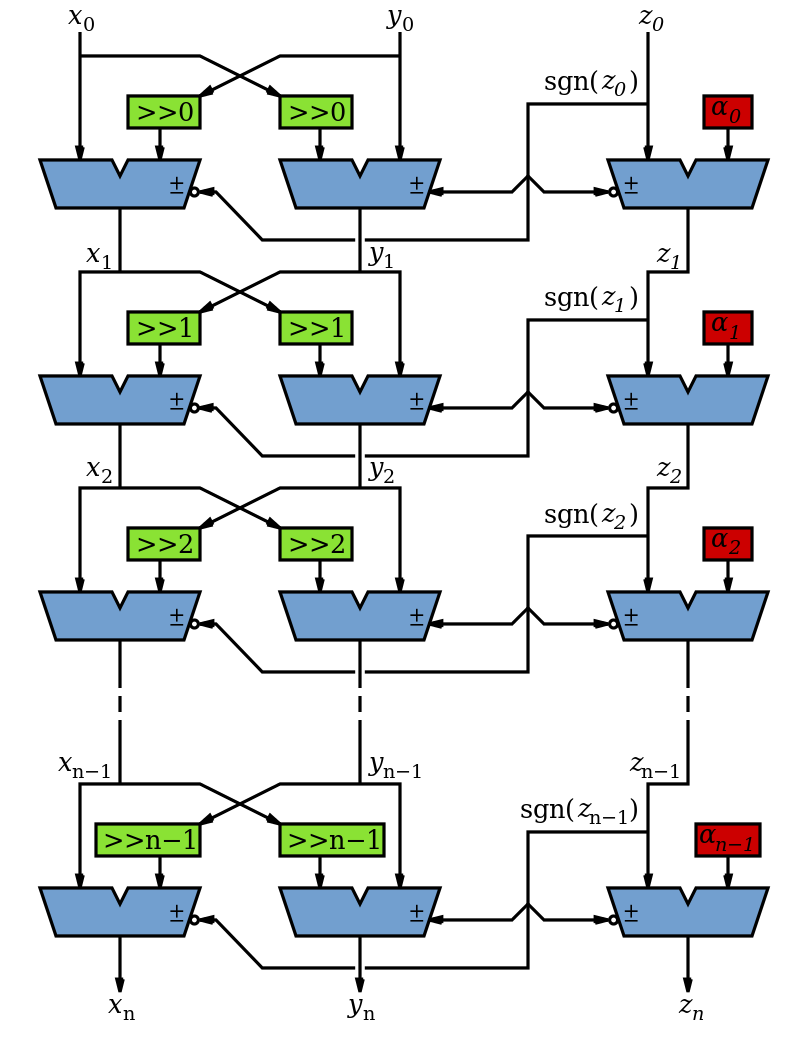
\includegraphics[width=0.7\textwidth]{images/6.png}
\end{figure}
and do more optimization \cite{wikicordic}.
\subsubsection{PYNQ Demo}
When streaming the output structs, the \textit{last} bit should be set to 1 for the last struct to be streamed, indicating end of stream. You may need to explicitly set the other \textit{last} bits to 0, otherwise your stream may terminate early and without warning since there may be garbage data at the memory addresses of the struct you create that are streamed out. You do not need to do this for inputs, as the tool takes care of it for you. Sometimes, the output streaming’s last bit is also handled by the tool, but sometimes it may not be, which will cause the DMA to hang (corresponding to a forever-running Jupyter cell) and it is better to hard code it.

Another point worth discussing here is why we use pointers for inputs and outputs, and why we have to post-increment the pointer manually when we stream inputs and outputs, but why it is a bad idea to use pointers in your code. You cannot use pointers in HLS; pointers are dynamic memory and Vitis HLS will not be able to synthesize it since it is not a deterministic thing (the datapath could change depending on inputs). Arrays, on the other hand, are fixed memory locations and therefore they can be synthesized to vectors in RTL. You can use pointers only as ports and even then you have to specify axistream, otherwise that will lead to synthesis issues as well.

In Vivado, the HP ports are High Performance ports which can be accessed by several interfaces. It is something like dynamic channel (also known as memory) which can access the entire channel at one go. Therefore it is not necessary to enable more than one HP port. This \href{https://forums.xilinx.com/t5/Processor-System-Design-and-AXI/MCDMA-or-Multiple-DMAs-Single-HP-port-or-Multiple-HP-ports/td-p/991992}{link} says to use two HP ports if you value performance. If you use multiple HP ports, in the memory map you can see this will give you more space to access (like 512M instead of 256M). So it is always safer to use separate ports although not required. You should have both DMAs be write-enabled (the lab had only one output, but here you have two outputs, so we’ll need both). If you choose to use more than one HP port, HP0 and HP1 should have different masters. So HP0 will have the first DMA as its master, and HP1 will have the second DMA. Two DMAs can point to a single HP port, but two HP ports cannot have the same DMA as master.

You also should see these outputs:
\begin{minted}{text}
Thetas at the R peaks are:
0.015529
0.047509
0.079485
0.111526
0.143491
...
\end{minted}
These are the rotated phases that have been detected by your design.
\subsubsection{Tasks}
In this project, you will build a phase detector to process the given complex signal (I and Q or real and imaginary parts) demonstrated in the figure below.
\begin{figure}[H]
    \centering
    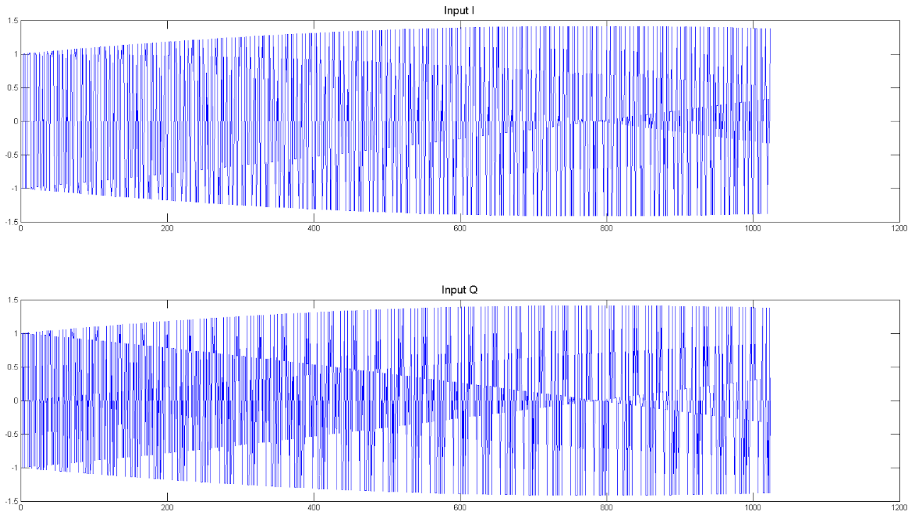
\includegraphics[width=\textwidth]{images/7.png}
\end{figure}
The final goal is to implement this phase detector. To achieve this goal, you will need to finish the following tasks:
\begin{enumerate}
    \item Design and verify a functionally complete CORDIC IP core using HLS: \texttt{cordic\_baseline}. You are provided a sample testbench that you can use though that the testbench does not cover all cases. You are required to create a more extensive testbench to ensure that your code is correct.
    \item Create an efficient CORDIC that only uses simple operations, i.e., add and shift. You should not be using divide, multiply, etc. in your CORDIC core. First design a baseline using float variables. Once you have a functionally correct CORDIC, then start experimenting with arbitrary precision data types. This should result in your multiplications being synthesized into shifts and adds (you should verify that this is indeed happening).
    \item A major design tradeoff for the CORDIC revolves around the precision or accuracy of the results. For example, changing the number of rotations effects the accuracy, performance, and resource usage. Another important tradeoff is the data type of the variables. Using large, complex data types (like floating point) is typically most accurate, but not good with respect to performance and resource usage. Fixed-point types provide better performance and resource usage, but may reduce the accuracy of the results. Perform design-space exploration to create a wide range of implementations using various data types for different variables, modifying the number of rotations, and performing other optimizations to find the Pareto optimal designs.
    \item Explore the architectural tradeoffs of a lookup table (LUT) architecture. We have provided a fully functional base implementation of this. You should read and understand this code. You should analyze the design-space of this lookup table IP core by changing the parameters of the look-up tables, e.g., by varying the data type of the input data and the output data types. This should allow you to find architectures with different resource usage, performance, and accuracy results.
    \item Implement the complex matched filter and verify it with the given testbench. This matched filter consists of four FIR filter modules which are similar to the ones in your Lab 3 Section 6.
    \item Connect the complex matched filter and CORDIC modules to implement the receiver. Verify this overall design with the given testbench.
    \item Modify this implementation code to gain better utilization or throughput.
    \item Implement the receiver design on the board. Plot the output data generated on board
    \begin{figure}[H]
        \centering
        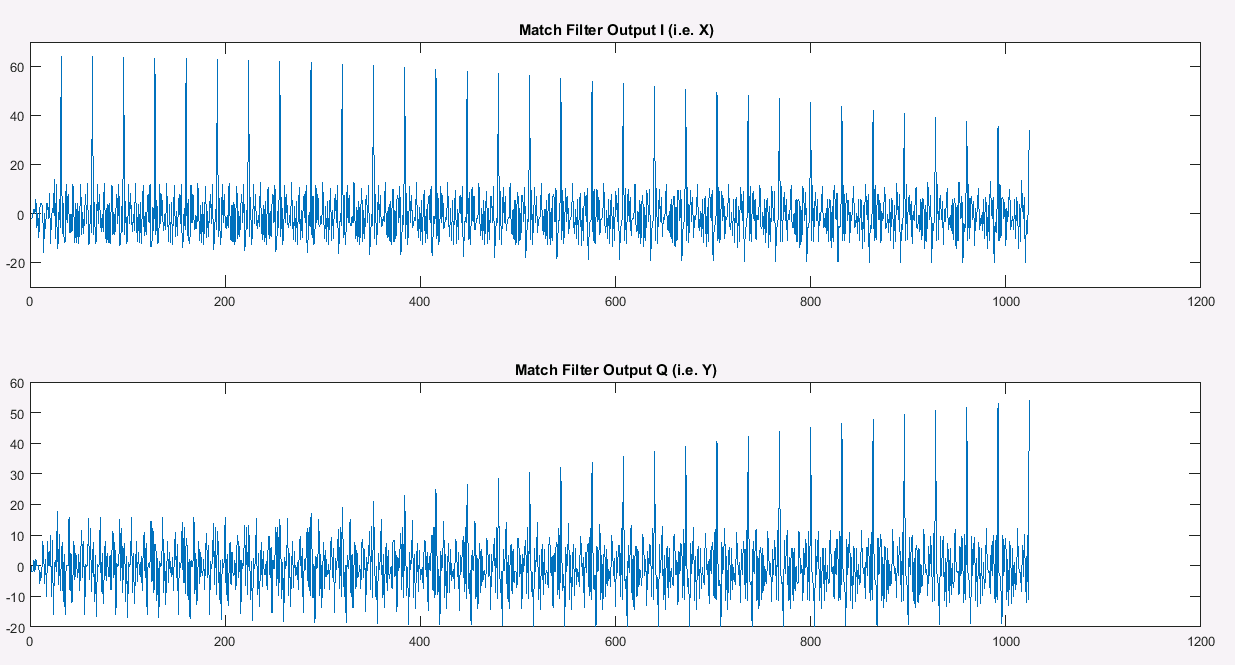
\includegraphics[width=\textwidth]{images/8.png}
    \end{figure}
    using \texttt{host.ipynb} or locally if using Vitis.
\end{enumerate}

\subsection{FFT and OFDM Receiver}
\subsubsection{Introduction}
In this project, you are supposed to learn the basic idea behind an orthogonal frequency-division multiplexing (OFDM) system by implementing a simple OFDM receiver in programmable logic. A major part of OFDM is a Fast Fourier Transform (FFT), and thus you will be working with your FFT implementation from the previous project. You are given a set of test benches for the different submodules. You should design and test each individual submodule individually and integrate them into the FFT module. In the final part of the project, you will complete the OFDM receiver by combining the FFT module with a QPSK symbol decoder.

The OFDM receiver is divided into two parts – the FFT and the QPSK decoder. You must design and implement a QPSK decoder and integrate it with the FFT to complete the receiver. While the major goal of this project is to create a functional core, you will also perform optimizations on the code.
\subsubsection{Fast Fourier Transform}
For the FFT part, the FFT implementation is divided into multiple stages. The first stage of the FFT reorders the input data using a bit reversal scheme. This gets added into a “software” version of the code that we have provided for you (minus the bit reversal portion). After that, you will create a more hardware-friendly FFT architecture. We have provided a set of testbenches for individual functions in addition to the testbenches for the overall FFT. While the major goal of this project is to create a functional core, you will also perform optimizations on the code. In particular, you have to achieve a target throughput in a final 1024-size FFT design that is less than 2000 clock cycles; therefore, with a ten ns clock period that is 50KHz. This can be achieved by optimizing the submodules properly and using dataflow pragma across the submodules.

The FFT is a more efficient version of the Discrete Fourier Transform (DFT). The FFT utilizes symmetry in the DFT coefficients to provide a recursive implementation that reduces the runtime from $O(N^2)$ to $O(N\log{N})$ where $N$ is the number of samples in the input signal.

The first step in most optimized FFT implementations is to reorder the input data by performing “bit reversed” swapping. This allows for in-place computation of the FFT, i.e., the resulting “frequency domain” data (as well as the intermediate results) can be stored in the same locations as the input “time domain” data. In addition, the output frequency domain data will be in the “correct order” at the end of the computation.

An example of the bit-reversed data for an 8-point FFT is as follows:
\begin{table}[H]
    \centering
    \begin{tabular}{|c|c|c|c|}
        \hline
        Input Decimal&Input Binary&Reversed Binary&Reversed Decimal\\
        Address&Address&Address&Address\\
        \hline
        0&000&000&0\\
        \hline
        1&001&100&4\\
        \hline
        2&010&010&2\\
        \hline
        3&011&110&6\\
        \hline
        4&100&001&1\\
        \hline
        5&101&101&5\\
        \hline
        6&110&011&3\\
        \hline
        7&111&111&7\\
        \hline
    \end{tabular}
\end{table}
In other words, the input data that was initially stored in the array at location 1 is stored in location 4 after the bit reversal is completed. The input data stored in the array at location 4 will be put in array location 1. The input data stored in locations 0, 2, 5, and 7 stay in those locations. Note that this is only true for an 8-point FFT. Other sizes of FFT will have different reordering of the data though it is still based on the bit reversed pattern. For example, in a 16-point FFT, the input data stored in location 1 (binary 0001) will be relocated into location 8 (binary 1000).

You should create an architecture that, efficiently as possible, transforms the input data into a bit reversed order. Note that there are many “software” implementations of this that will not effectively map to “hardware”. While the first goal is to get a working function, you should also consider the performance of the architecture.

We have given you a set of files that allows you to develop and test this bit reversal code in isolation. This includes a simple testbench that exercises this function directly. You should develop and optimize your bit-reversed code here. You will later copy this code into the FFT code. The bit reverse function has the following prototype: \verb|void bit_reverse(DTYPE X_R[SIZE], DTYPE X_I[SIZE])|. You should perform the swapping “in place” on the data in both of the real and imaginary portions of the data. That is the input data in both X\_R and X\_I will be reordered when the function completes. Focus on how you modified your code in order to make it more “hardware friendly”.

The next portion of this project performs optimization on a typical software implementation of the FFT. You are given a typical three-nested loop implementation of the FFT in the folder 0\_Initial. First, you should understand in detail what this code is doing. It is worth spending time on this now as you will have to rewrite the FFT in a more hardware-friendly manner in the next steps. You can reuse some of this code in those steps.

You should optimize this code as much as possible. The results of the code will be poor; it will likely have > 250 million cycles. The throughput here is likely much worse than running this in software on a microprocessor. This often happens when we put the initial software versions of an application into a high level synthesis tool. And it should not be all that surprising. The code is optimized to run quickly in software, which runs largely in a sequential model of computation. The code must typically be carefully optimized with the final hardware architecture in mind to get good results. This involves exploiting parallelism and pipelining.

Some potential optimizations include:
\begin{itemize}
    \item Using the W\_real and W\_imag tables
    \item Pipelining
    \item Loop unrolling
    \item Memory partitioning
\end{itemize}
A good architecture will selectively expose and take advantage of parallelism and allow for pipelining. Your final FFT architecture will restructure the code such that each stage is computed in a separate function or module. There will be one module for bit reversal that you have already developed, and then log N stages (10 in our case) for the butterfly computations corresponding to the 2-point, 4-point, 8-point, 16-point, … FFT stages.

The skeleton code for this final FFT implementation can be found in the 2\_Skeleton\_Restructured folder. This creates code that connects a number of functions in a staged fashion, with arrays acting as buffers between the stages. Figure \ref{FFFT} provides a graphical depiction of this process.
\begin{figure}[H]
    \centering
    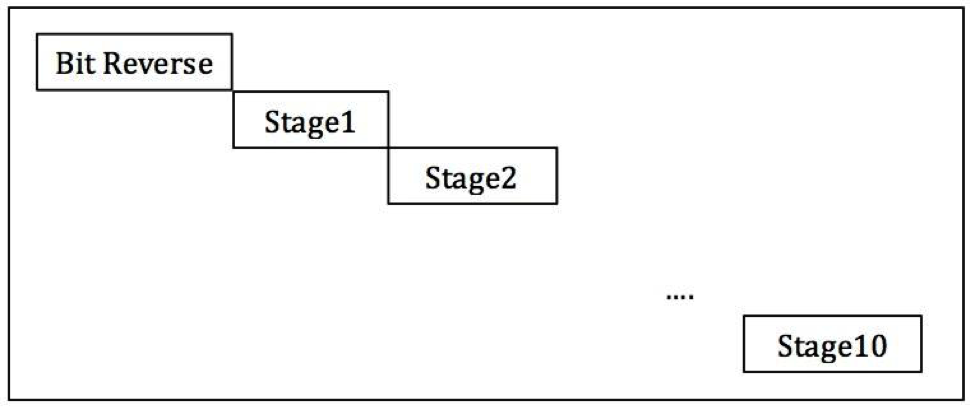
\includegraphics[width=\textwidth]{images/9.png}
    \caption{A staged implementation of a 1024 FFT. Bit reversal is followed by ten stages of butterfly computations. This architecture is capable of pipelines both within stages and across the stages.}
    \label{FFFT}
\end{figure}
The first step in this process is to create code that computes the first and last stages of the FFT. The hope is that this will allow you to get a better understanding of exactly how memory accesses and the butterfly computations are performed in a general case. You can develop these two functions fft\_stage\_first and fft\_stage\_last in isolation. They both have subfolders in the 1\_Subcomponents folder. Once these are working correctly, you can copy and paste the code directly into the same functions in the 2\_Skeleton\_Restructured project.

The next task is to create code that can implement a “generic” function, i.e., one that can compute any stage of the FFT. This is the function fft\_stages which also has its own project in the 1\_Subcomponents folder. Note that this function prototype is similar to fft\_stage\_first and fft\_stage\_last with one major difference: it has a "stage" argument. This code will be used to implement stages 2 through 9 in the 2\_Skeleton\_Restructured project.

These stages perform the same calculation as one iteration of the outer for loop in the 0\_Initial project. The major difference between the stages is what data elements you are performing the butterfly functions on, i.e., in what order do you pull data from X\_R and X\_I. Test each of the functions in isolation with the provided projects. Make sure that the code compiles and passes the testbench before attempting any optimizations.

Once you have a correctly functioning set of functions, you should copy and paste them into the 2\_Skeleton\_Restructured project and make sure that it passes the testbench. The sample testbenches on perform one check, which is far from comprehensive, it is possible, though hopefully unlikely, that you have some error that the 2\_Skeleton\_Restructured testbench exposes and was not exercised in the individual testbench. You need to perform significantly more testing in any “non-class” situation).

To optimize the restructured code, you should perform the typical tricks here: pipelining, memory partitioning, unrolling, etc. Some of these may not make sense, depending on how you wrote your code. This final architecture should be orders of magnitude better than the 0\_Initial project. Highly optimized FFT architectures can easily have less than 10000 cycles.

You must always use a clock period of 10 ns.
\subsubsection{QPSK Decoder}
The decoder takes the output of the FFT (complex values) and translates them into data. This is essentially undoing the effect of the QPSK encoder, which takes input data for transmission and encodes it into a complex exponential, i.e., an I/Q complex number. You can think of this as a translation from the input data into a complex number.

We used the QPSK encoding scheme shown in the below figure. The plot shows four points in the complex plane at (+- 0.707, +- 0.707). This is called a constellation. Each of these points is labeled with an integer value 0, 1, 2, or 3. These integer values corresponding to the input data being encoded. You can also think of these as two-bit values if you want to consider binary input data. The complex values are the I/Q data that is encoded onto a specific frequency (e.g., one of 1024 frequencies when using a 1024-point FFT). The decoder performs the opposite – it takes a complex number and translates it into an integer. You can look at the Simulink file for more information. This figure is taken directly from that file. The output of your encoder should be the exact data that was given to the OFDM receiver in the Simulink file.
\begin{figure}[H]
    \centering
    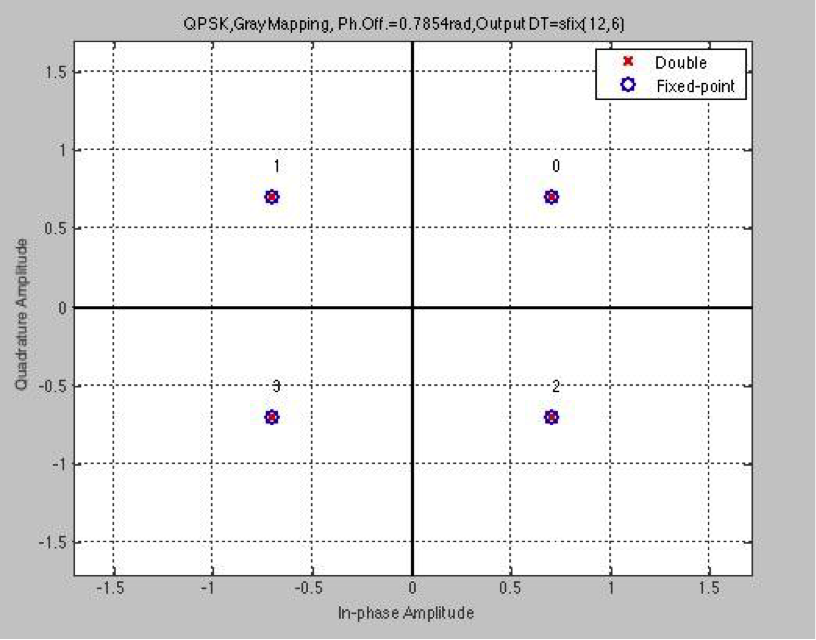
\includegraphics[width=\textwidth]{images/10.png}
\end{figure}
You should connect the FFT and the QPSK decoder together to form the complete OFDM receiver. The input to the receiver is the data from the channel. The output of the receiver should match the transmitted data. You must always use a clock period of 10 ns.
\subsubsection{Tasks}
Your tasks for this part of the project are:
\begin{enumerate}
    \item Implement a working FFT module that passes the testbench in HLS.
    \item Optimize the FFT module to achieve a target throughput
    \item Implement the QPSK decoder.
    \item Integrate the FFT and decoder into a complete OFDM receiver.
    \item Integrate the receiver onto the Zynq’s processing system (PS) using a proper interface to transmit data to the OFDM receiver and receive the decoded data back from your hardware implementation on the Zynq’s programmable logic (PL). Write a host Pynq Jupyter Notebook or a Vitis application for evaluation.
\end{enumerate}

\subsection{MLP Neural Network}
\subsubsection{Introduction}
The goal of this project is to create a hardware accelerator for a multilayer perceptron neural network. A multilayer perceptron (MLP) is a class of feedforward artificial neural networks. An MLP consists of at least three layers of nodes: an input layer, a hidden layer, and an output layer. Except for the input nodes, each node is a neuron that usually uses a nonlinear activation function. MLP utilizes a supervised learning technique called backpropagation for training. MLP can also be trained using other techniques such as Genetic Algorithms, Particle Swarm Optimization, etc.

We will be implementing the hardware accelerator for prediction, not for training. Training the neural network (which involves optimizing the weights of the connections in the network to minimize prediction error) can be done separately on a PC / Laptop, and the weights can be stored in a file. For the sample data given on this page, the training is already done, and the weights are provided. Implementing the architecture mentioned below and using these weights is good enough to meet the basic requirements. Even if you are using a different neural network architecture or dataset, the training can still be done offline.

To implement prediction (predicting the label of a new input data), there are three different ways
\begin{enumerate}
    \item SOFT: A pure software implementation on the ARM Cortex A9.
    \item HARD\_HDL: An AXIS co-processor implementing the neural network in hardware, written in HDL. This should be able to receive the weights and the data from the software running on ARM Cortex A9 and return the predicted labels.
    \item HARD\_HLS: An AXI / AXI Lite / AXIS co-processor implementing the neural network in hardware, which is at least partly created using the HLS tool. This should be able to receive the weights and the data from the software running on ARM Cortex A9 and return the predicted labels. 
\end{enumerate}
In this project, you are only required to implement HARD\_HLS.
\subsubsection{Procedure}
You will send the data from the PC via the serial console (PuTTY, Vitis Serial Terminal, etc.). It is fine to hardcode the size of the data in your program; however, the data itself should be sent via the serial console.

The C program running on the ARM Cortex A9 processor should receive the dataset, get the prediction done through HARD\_HLS, and send the predictions back to the console. This can be captured in a file, which can then be compared against the actual labels to compute the prediction accuracy (using, say, Excel).

The weights can be hard-coded in the C program or sent from the PC, but it should not be hard-coded in your coprocessor design, i.e., the coprocessor should be able to deal with different weights. This allows the same coprocessor (hardware) to deal with possibly different datasets and weights, provided the neural network architecture and data dimensionality does not change. At least, the data dimensionality should not exceed what you had designed for, i.e., 7. A lower-dimensional data can be easily dealt with by setting the weights corresponding to unused features to 0. A dataset that has more samples/data points can be dealt with by having an appropriate C program that can break it into chunks that the coprocessor can accept, which is 64 in our case.

You can make your own choices regarding the neural network architecture, such as the number of hidden layers, the number of neurons in each hidden layer, etc., subject to some minimum requirements:
\begin{itemize}
    \item There should be at least one hidden layer.
    \item There should be at least two neurons in the hidden layer(s) using a non-linear activation function that is not piecewise linear (e.g., not ReLU or variants).
    \item There are no restrictions regarding the activation functions used elsewhere, i.e., the third neuron onwards in the hidden layer or in additional hidden layers. 
\end{itemize}
The sample data section below has data and pre-trained weights for the neural network architecture described in that section, which is enough to meet the basic requirements. You are free to explore other architecture and/or other data. The focus, though, is on exploring hardware architectures rather than exploring different neural network architectures - the module is on hardware design, and machine learning just happens to be the application we chose to accelerate (which we thought would give many who are new to machine learning some flavor of it).

Having said that, exploring some hardware-related aspects (such as dealing with overflows, negatives, precision issues, etc.) wouldn't be possible with the pre-trained network above - you will have to do your own training for that.

It is not just about getting things functionally/algorithmically correct. It is about having a systematic design and being able to appreciate the various tradeoffs. There is no fixed requirement regarding the accuracy or resource usage, or performance - all these are interdependent. Your design should be Pareto-optimal, i.e., it should be such that one figure of merit cannot be improved without compromising on another.
\subsubsection{Sample data}
You can use any dataset you like. A synthetic dataset (a distorted version of the original wine dataset), as well as the weights for the neural network, are given below.

The input layer has seven nodes, corresponding to 7 features. The matrix contained in X.csv is a 64 x 7 matrix, corresponding to 64 data points, each with seven features.

There is one hidden layer having two neurons, with the neurons having 1 (decimal) as bias input (you can consider this as 255 or 256 as you wish in the 0.8 unsigned fixed-point formats we use). In other words, we do $\frac{\sum_0^7{w_i\times x_i}}{256}$ where $w_0$ is the bias and $x_0$ is considered 255 or 256. Why is 256 ok when it doesn't fit into 8 bits? Because 256 (representing 1.0) can be implicitly used by doing << 8 (which can be done by appropriate bit wiring) instead of multiplication. Alternatively, you can simply do $w_0+\frac{\sum_1^7{w_i\times x_i}}{256}$. Please keep in mind the representation format, and things will be clearer.

The neurons in the hidden layer have a sigmoid activation function, as given below. The exact formula used is  $y=256\cdot\frac{1}{1+e^{-\left(\frac{6x}{256}-3\right)}}$, where x is an integer in the interval [0, 255], i.e., $x$ is in the 0.8 formats. This uses only the middle part of the curve, so the amount of non-linearity is not very high.
\begin{figure}[H]
    \centering
    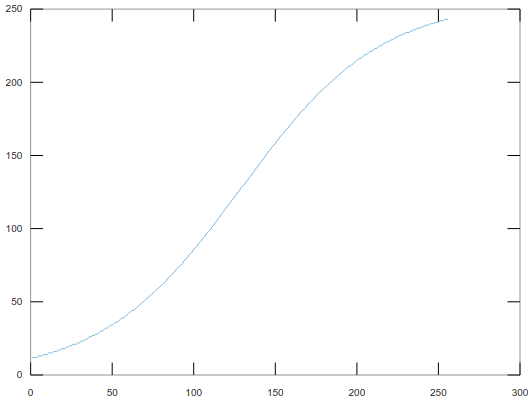
\includegraphics[width=\textwidth]{images/11.png}
\end{figure}
The sigmoid function can be computed using a lookup table given in \texttt{sigmoid.csv}. The input to the function is used as an index to look up the output of the function. It is also fine to compute it directly using the formula if you wish.

The file \texttt{w\_hid.csv} contains the weights for the hidden layer. This is an 8 x 2 matrix, with the first row containing the weight for the bias term and the rest of the seven rows containing weights for each of the features. The two columns represent the weights corresponding to the two neurons in the hidden layer.

The output layer has a bias input too, and a linear activation function, i.e., the output is simply the weighted sum of inputs to the neurons (and bias). The 3 x 1 weight matrix is given in \texttt{w\_out.csv}, where the first element is the weight of the bias term, and the rest of the two are weights for the outputs from the hidden later.

The labels for verification can be found in \texttt{labels.csv}.

Note: In unsigned 0.8 fixed-point formats, there is an implicit scale factor of 256. So whenever you have a multiplication of two 0.8 format numbers, you need to scale down by 256. Whenever you have a division, you should scale up by 256. Addition and subtraction don't change the scale. When you are doing multiply and accumulate, you can do the scaling down by 256 after accumulation, which will preserve precision better than scaling down after every single multiplication.

You can refer to \cite{bppdf}.
\subsection{SRAM Generator}
\subsubsection{Introduction}
Small memories can be easily synthesized using flip-flops or latch standard cells, but synthesizing large memories can significantly impact the area, energy, and timing of the overall design. ASIC designers often use SRAM generators to “generate” arrays of memory bitcells and the corresponding peripheral circuitry (e.g., address decoders, bitline drivers, sense amps), which are combined into what is called an “SRAM macro”. These SRAM generators are parameterized to enable generating a wide range of SRAM macros with different numbers of rows, columns, and column muxes, as well as optional support for partial writes, built-in self-test, and error correction. Similar to a standard-cell library, an SRAM generator must generate not just layout but also all of the necessary views to capture logical functionality, timing, geometry, and power usage. These views can then be used by the ASIC tools to produce a complete design that includes a mix of both standard cells and SRAM macros. We will first see how to use the open-source OpenRAM memory generator to generate various views of an SRAM macro. Then we will see how to use SRAMs in our RTL designs. Finally, we will put these two pieces together to combine synthesizable RTL with SRAM macros and push the composition through the ASIC toolflow.

The following diagram illustrates how the memory generator integrates with the four primary tools covered in the previous labs. We run the memory generator to generate various views, which are then combined with the standard cell views to create the complete library used in the ASIC flow.
\begin{figure}[H]
    \centering
    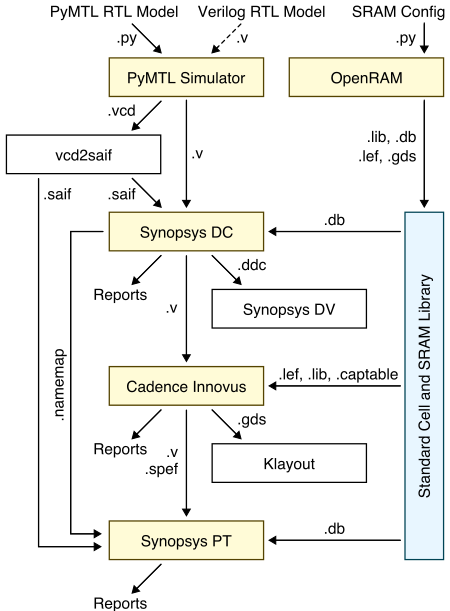
\includegraphics[width=0.7\textwidth]{images/12.png}
\end{figure}
\subsubsection{OpenRAM Memory Generator}
Just as with standard-cell libraries, acquiring real SRAM generators is a complex and potentially expensive process. It requires gaining access to a specific fabrication technology, negotiating with a company that makes the SRAM generator, and usually signing multiple non-disclosure agreements. The OpenRAM memory generator is based on the same “fake” 45nm technology that we are using for the Nangate standard-cell library. The “fake” technology is representative enough to provide reasonable area, energy, and timing estimates for our purposes. In this section, we will take a look at how to use the OpenRAM memory generator to generate various views of an SRAM macro.

You can see an example configuration file for the OpenRAM memory generator from \texttt{SRAM\_32x128\_1rw.py}.

In this example, we are generating a single-ported SRAM that has 128 rows and 32 bits per row for a total capacity of 4096 bits or 512B. This size is probably near the cross-over point where you might transition from using synthesized memories to SRAM macros. OpenRAM will take this configuration file as input and generate many different views of the SRAM macro, including schematics (.sp), layout (.gds), a Verilog behavioral model (.v), abstract logical, timing, power view (.lib), and a physical view (.lef). These views can then be used by the ASIC tools.

You can find more information about the OpenRAM memory generator in this recent research paper: \cite{10.1145/2966986.2980098}.

The following excerpt from the paper illustrates the microarchitecture used in the single-port SRAM macro in the original OpenRAM implementation.
\begin{figure}[H]
    \centering
    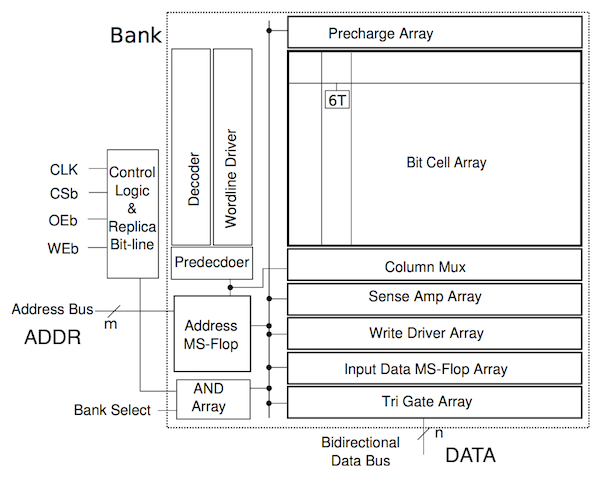
\includegraphics[width=\textwidth]{images/13.png}
\end{figure}
The functionality of the pins is as follows:
\begin{itemize}
    \item \texttt{clk}: clock
    \item \texttt{WEb}: write enable (active low)
    \item \texttt{OEb}: output enable (active low)
    \item \texttt{CSb}: whole SRAM enable (active low)
    \item \texttt{ADDR}: address
    \item \texttt{DATA}: read/write data
\end{itemize}
Notice that there is a single address and a single read/write data bus. This SRAM macro has a single read/write port and only supports executing a single transaction at a time. The following excerpt from the paper shows the timing diagram for a read-and-write transaction.
\begin{figure}[H]
    \centering
    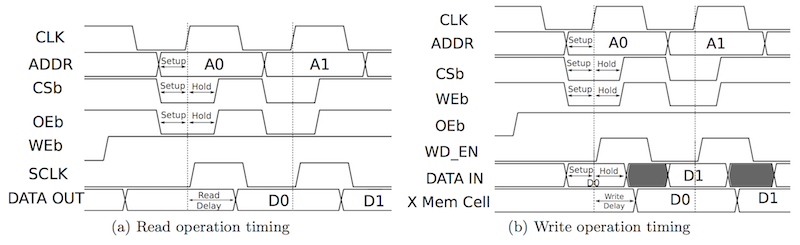
\includegraphics[width=\textwidth]{images/14.png}
\end{figure}
In order to execute any kind of transaction in the SRAM, we need to set the \texttt{CSb} pin low (note that \texttt{CSb} is active low). Let’s start by focusing on the read transaction shown on the left. For the read transaction on the left, the \texttt{WEb} pin is set high (note that \texttt{WEb} is active low). The \texttt{ADDR} pins are used to set the row address. Note that this is a row address, not a byte address. From the block diagram, we can see that the address first goes into the “Address MS-Flop”. This is an array of flip-flops that store the address on the rising edge of the clock. After the rising edge, the address is decoded to drive the word lines and enable the desired row. The read data is driven from the bit cell array through the column muxing and into the sense amp array. The \texttt{OEb} pin was used to determine whether the read data should be driven onto the data bus. This can enable multiple SRAM macros to be arranged on a distributed bus with only one SRAM driving that bus on any given cycle. The \texttt{OEb} pin has since been removed in OpenRAM, and its functionality was tied to the \texttt{CSb} pin. Assuming \texttt{CSb} is low, then the read data is driven out the \texttt{DATA} pins. Since we set the address before the edge and the data is valid after the edge, this is a synchronous read SRAM. Compare this to a register file which often provides a combinational read where the address is set, and the data is valid sometime later during the same cycle. Most SRAM generators produce synchronous read SRAM macros. For the write transaction on the right, the WEb pin is set low, and the \texttt{DATA} pins are driven with the write data.
\subsubsection{Using SRAMs in RTL Models}
There is both a PyMTL and Verilog version. Both are parameterized by the number of words and the bits per word, and both have the same pin-level interface:
\begin{itemize}
    \item \texttt{port0\_val}: port enable
    \item \texttt{port0\_type}: transaction type (0 = read, 1 = write)
    \item \texttt{port0\_idx}: which row to read/write
    \item \texttt{port0\_wdata}: write data
    \item \texttt{port0\_wben}: write byte enable
    \item \texttt{port0\_rdata}: read data
\end{itemize}
SRAMs use a latency \textit{sensitive} interface meaning a user must carefully manage the timing for correct operation (i.e., set the read address and then exactly one cycle later use the read data). In addition, the SRAM cannot be “stalled”. To illustrate how to use SRAM macros, we will create a latency \textit{insensitive} minion wrapper around an SRAM, which enables writing and reading the SRAM using our standard memory messages. The following figure illustrates our approach to implementing this wrapper:
\begin{figure}[H]
    \centering
    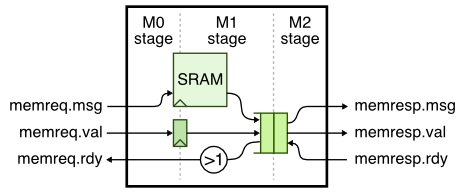
\includegraphics[width=\textwidth]{images/15.png}
\end{figure}
Here is a pipeline diagram that illustrates how this works.
\begin{minted}{text}
cycle : 0  1  2  3  4  5  6  7  8
msg a : M0 Mx
msg b :    M0 Mx
msg c :       M0 M1 M2 M2 M2       # M2 stalls on cycles 3-5
msg d :          M0 M1 M1 M1 M2    # but wait, we cannot stall in M1!
msg e :             M0 M0 M0 M0 Mx

cycle M0 M1 [q] M2
   0: a
   1: b  a      a  # a flows through bypass queue
   2: c  b      b  # b flows through bypass queue
   3: d  c         # M2 is stalled, c will need to go into bypq
   4: e  d   c     # q is full at beginning of cycle, enq_rdy = 0
   5: e  ?   c     # what happens to d? cannot stall in M1!
\end{minted}
Here we are using Mx to indicate when a transaction goes through M1 and M2 in the same cycle because it flows straight through the bypass queue. So on cycle 3, the response interface is stalled, and as a consequence, message c must be enqueued into the memory response queue. On cycle 4, the response queue is full (\texttt{recv\_rdy} = 0) so \texttt{memreq\_rdy} = 0, and message e will stall in M0 (i.e., will stall waiting to be accepted by the SRAM wrapper). The critical question is, what happens to message d? It cannot stall in M1 because we \textit{cannot} stall the SRAM. So basically, we just drop it. Increasing the amount of buffering in the bypass queue will not solve the problem. The key issue is that by the time we realize the bypass queue is full, we can potentially already have a transaction executing in the SRAM, and this transaction cannot be stalled.

This is a classic situation where the need more skid buffering. A correct solution will have two or more elements of buffering in the memory response queue and stall M0 if there are fewer than two free elements in the queue. Thus in the worst case, if M2 stalls, we have room for two messages in the response queue: the message currently in M1 and the message currently in M0. Here is the updated design:
\begin{figure}[H]
    \centering
    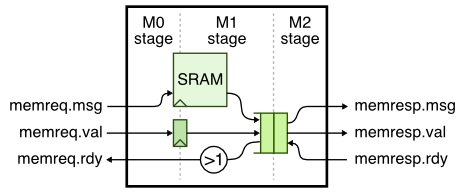
\includegraphics[width=\textwidth]{images/16.png}
\end{figure}

\subsubsection{Tasks}
\begin{enumerate}
    \item Experiment with the configuration file to generate other SRAM macros and report your discovery on generated behavioral Verilog, transistor-level netlist, actual layout from a macroscopic and microscopic perspective, and SRAM macro library.
    \item Create \texttt{SRAM\_128x256\_1rw-cfg.py}, \texttt{SRAM\_128x256\_1rw.py}, and \texttt{SRAM\_128x256\_1rw.v} with \texttt{words\_per\_row} = 4.
    \item Create a new SRAM configuration file \texttt{SRAM\_32x128\_1rw-cfg.py}.
    \item Create an SRAM configuration RTL model \texttt{SRAM\_32x128\_1rw.py} and \texttt{SRAM\_32x128\_1rw.v}.
    \item Use new SRAM configuration RTL model in top-level SRAM model and complete \texttt{SramPRTL.py} and \texttt{SramVRTL.v}
    \item Complete \texttt{SramMinionPRTL.py} and \texttt{SramMinionVRTL.v} TODO and PROJECT TASKS sections.
    \item Test new SRAM configuration by \texttt{pytest}, and complete \texttt{SramRTL\_test.py}.
    \item Choose Verilog or PyMTL3 to generate the SRAM macro.
    \item Convert the \texttt{.lib} file into a \texttt{.db} file using the Synopsys Library Compiler (LC) tool.
    \item Run the full ASIC flow on the SRAM to produce an optimized valid design. You can optionally use \texttt{mflowgen} to accelerate your ASIC flow.
    \item Compare $32\times256$ SRAM, $128\times256$ SRAM, and $32\times128$ SRAM.
\end{enumerate}

\subsection{ASIC Integer Multiplier}
\subsubsection{Introduction}
In Lab 2 Section 5, you optionally practiced the pipelined integer multiplier on FPGA. In this project, you will use a standard-cell ASIC toolflow to quantitatively analyze the area, energy, and performance of various integer multiplier designs. You will push three given baseline designs through the ASIC toolflow: a fixed-latency iterative design that always takes the same number of cycles, a variable-latency iterative design that exploits properties of the input operands to reduce the execution time, and a simple single-cycle design. The alternative design is a pipelined integer multiplier that is parameterized by the number of pipeline stages. You are required to implement both a register-transfer-level (RTL) model of the alternative design, verify the design using an effective testing strategy, push all designs through the ASIC toolflow, and perform an evaluation comparing the various implementations. Your experience in this project will create a solid foundation for ASIC flow.

All of the tests should pass except for the tests related to the multipliers you will be implementing in this lab.

In previous labs, you learned how to evaluate baseline and alternative designs according to several key metrics: execution time (in cycles), area, energy, and cycle time. Using RTL modeling, we were able to quantitatively measure the execution time (in cycles) for a given input dataset for each design, but we relied on qualitative estimates to analyze the area, energy, and cycle time of each design. In this project, we will learn how to use a standard-cell ASIC toolflow to quantitatively measure the area, energy, and cycle time of a design; we can then combine these measurements with our understanding of the cycle-level performance of each design to conduct a much more detailed design-space exploration.

We have provided you with a functional-level model of an integer multiplier. You can find this functional-level (FL) implementation in \texttt{IntMulFL.py} and the associated unit tests in \texttt{test/IntMulFL\_test.py}. This implementation verifies the functionality and uses a higher-level modeling style compared to register-transfer-level (RTL) modeling. The interface for the FL model and, indeed, for all of the integer multiplier designs are similar in that they accept two 32-bit numbers and produce a single 32-bit multiplication result. All implementations should treat the input operands and the result as two’s complement numbers and thus should be able to handle both signed and unsigned multiplication. The FL model is a simple Python function, and the RTL model uses port-based interfaces and the val/rdy micro-protocol. By leveraging the val/rdy micro-protocol, another module would be able to send request messages to the multiplier and never explicitly be concerned with how many cycles
the implementation takes to execute a multiply transaction and return the response message.
\begin{figure}[H]
    \centering
    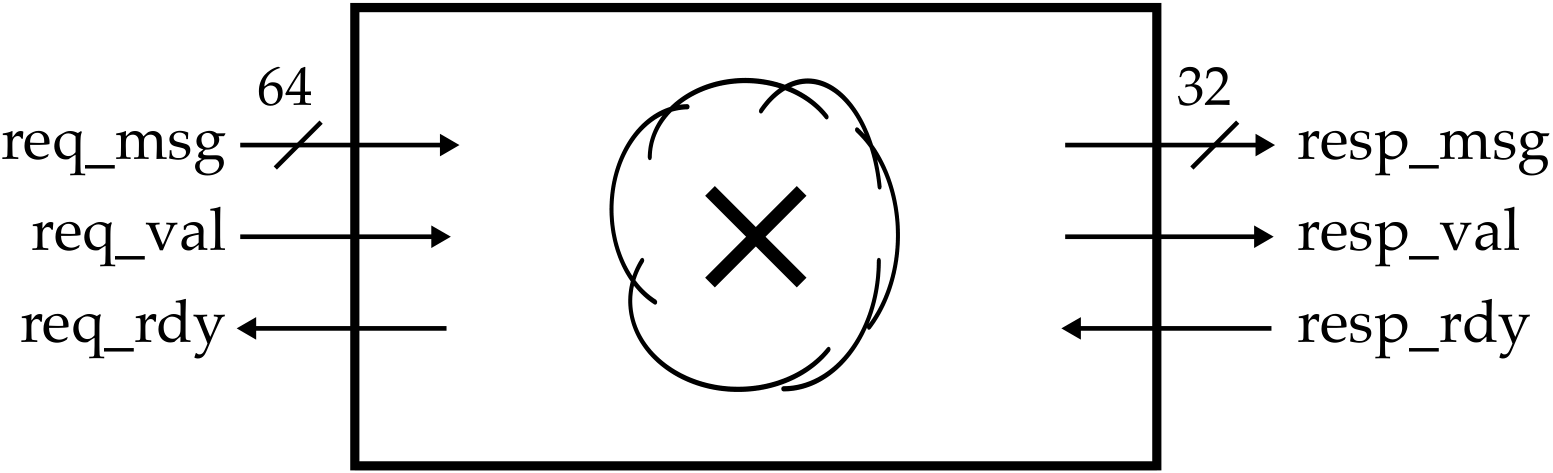
\includegraphics[width=\textwidth]{images/17.png}
    \caption{RTL Integer Multiplier Interface – RTL model uses port-based interfaces leveraging val/rdy micro-protocol.}
    \label{F17}
\end{figure}
\subsubsection{Baseline Design}
There are three baseline designs for this lab assignment: a fixed-latency iterative integer multiplier, a variable-latency iterative multiplier, and a simple single-cycle multiplier. The RTL models of each design are provided for you. All baseline designs use the same interface shown in Figure \ref{F17}.
\begin{listing}[H]
\begin{minted}{python}
def imul_fixed_algo( a, b ):

    result = Bits( 32, 0 )
    for i in range(32):
        if b[0] == 1:
            result += a
        a = a << 1
        b = b >> 1
        
    return result
\end{minted}
\caption{Fixed-Latency Iterative Multiplication Algorithm – Assumes a and b are 32-bit Bits objects. Always uses 32 shifts and subtractions to calculate the partial products over time. This is executable Python code.}
\label{L2}
\end{listing}
The fixed-latency iterative multiplier will always take approximately 32 cycles. Listing \ref{L2} illustrates the fixed-latency iterative multiplication algorithm using “pseudocode,” which is really executable Python code. For each iteration, we check the least significant bit of the b operand; if this bit is zero, then we shift the \texttt{b} operand to the right and the \texttt{a} operand to the left, but if this bit is one then we add a to the result before shifting. Each iteration is essentially calculating a partial product for the multiplication. Note that we say “approximately” because there may be a few extra cycles of overhead in handling the val/rdy micro-protocol (although a more optimized design can remove this overhead).
\begin{figure}[H]
    \centering
    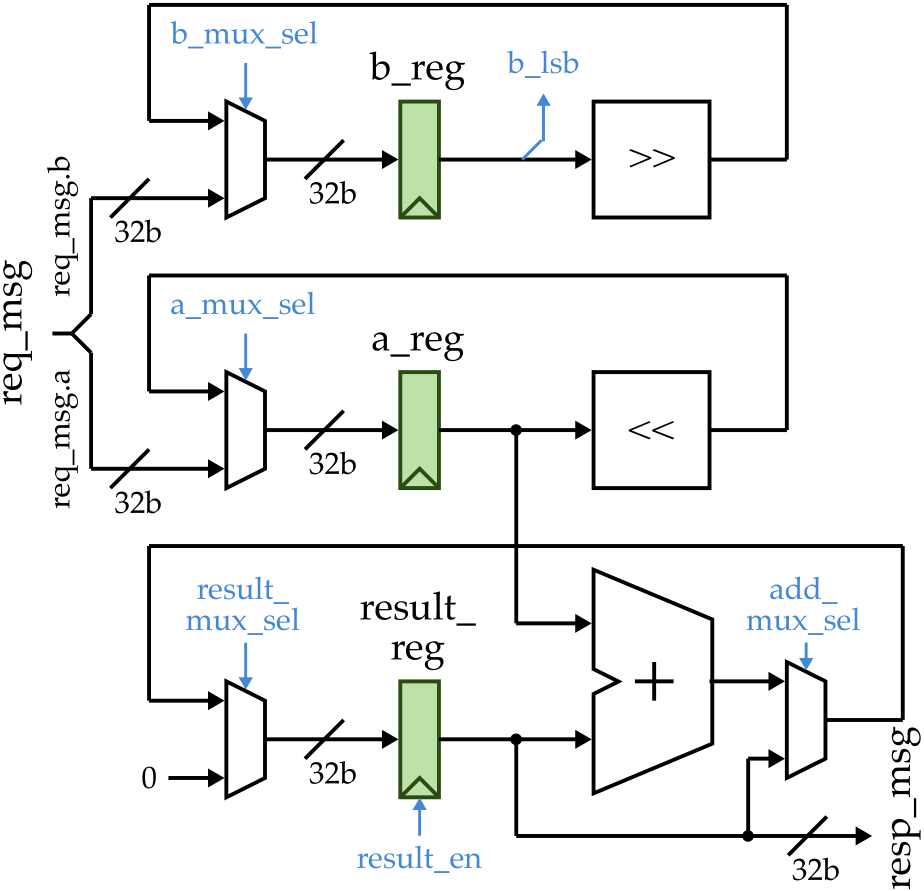
\includegraphics[width=0.6\textwidth]{images/18.png}
    \caption{Datapath for Fixed-Latency Iterative Integer Multiplier – All datapath components are 32-bits wide. Shifters are constant one-bit shifters. We use registered inputs with a minimal of logic before the registers.}
    \label{F18}
\end{figure}
The fixed-latency iterative multiplier RTL model uses a control/datapath split. The datapath for the fixed-latency design is shown in Figure \ref{F18}. The blue signals represent control/status signals for communicating between the datapath and the control unit. The datapath model uses a structural design style by instantiating a child module for each of the blocks in the datapath diagram. The control unit for the fixed-latency design uses the simple finite-state machine shown in Figure \ref{F19}. The IDLE state is responsible for consuming the message from the input interface and placing the input operands into the input registers; the CALC state is responsible for iteratively using adds and shifts to calculate the multiplication, and the DONE state is responsible for sending the message out the output interface. Note that if you implement the FSM precisely as shown, each multiply should take 35 cycles: one for the IDLE state, 32 for iterative calculation, one cycle to realize the calculation is done, and one cycle for the DONE state. The extra cycle to realize the calculation is done is because we are not using Mealy transitions from the CALC to DONE states. We need to wait for the counter to reach 32, and then we move into the idle state. The control unit is structured into three parts: a sequential, concurrent block for just the state element, a combinational concurrent block for state transitions, and a combinational concurrent block for state outputs. The PyMTL code for the fixed-latency iterative multiplier RTL model is in IntMulFixedLatPRTL.py, and the Verilog code is in IntMulFixedLatVRTL.v.
\begin{figure}[H]
    \centering
    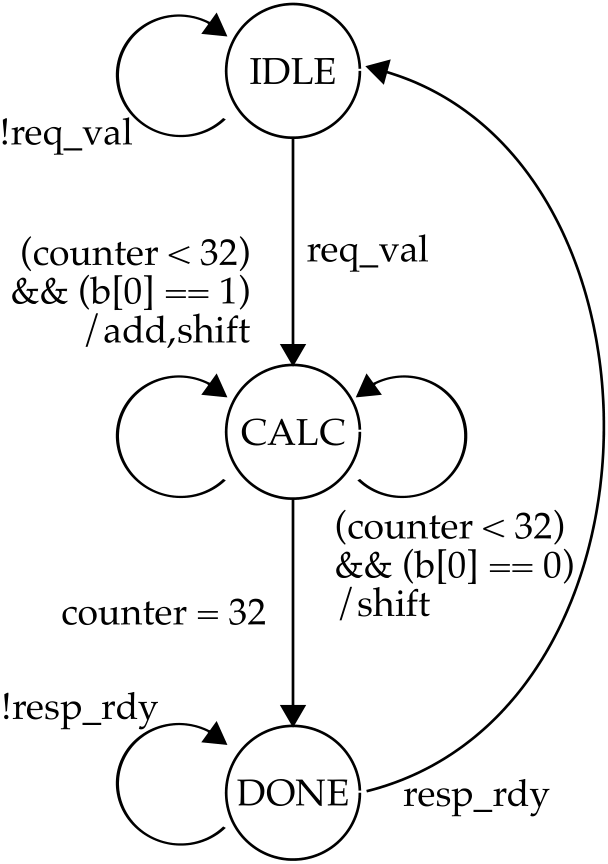
\includegraphics[width=0.5\textwidth]{images/19.png}
    \caption{Control FSM for Fixed-Latency Iterative Integer Multiplier – Hybrid Moore/Mealy FSM with Mealy transitions in the CALC state.}
    \label{F19}
\end{figure}
The fixed-latency iterative integer multiplier will always take 35 cycles to compute the result. While it is possible to optimize away the cycle to realize the calculation is done and to eliminate the IDLE/-DONE states, fundamentally, this algorithm is limited by the 32 cycles required for the iterative calculation. The variable-latency iterative multiplier takes advantage of the structure in some pairs of input operands to improve performance and energy efficiency. Listing \ref{L3} illustrates the variable-latency iterative multiplication algorithm using “pseudocode”. If the b operand has many consecutive zeros, we don’t need to shift one bit per cycle; instead, we can shift the B register multiple bits in one step and directly jump to the next required addition. The \texttt{calc\_shamt} function calculates the shift amount based on the number of trailing zeros in the b operand. Various different implementations of \texttt{calc\_shamt} are possible: considering more bits will improve the performance but likely increase area and energy.
\begin{listing}[H]
\begin{minted}{python}
def imul_var_algo( a, b ):

    result = Bits( 32, 0 )
    while b != 0:
        if b[0] == 1:
            result += a
        shamt = calc_shamt( b )
        a = a << shamt
        b = b >> shamt
        
    return result
\end{minted}
\caption{Variable-Latency Iterative Multiplication Algorithm – Assumes a and b are 32-bit Bits objects. Shifts
by more than one to skip over sequences of zeros in the b operand. Various different \texttt{calc\_shamt} functions are possible. This is executable Python code.}
\label{L3}
\end{listing}
The variable-latency iterative multiplier RTL model is very similar to the fixed-latency RTL model with a couple of key differences. The datapath for the variable-latency design is shown in Figure \ref{F20}. Notice that we have added a new model that takes the b operand and input and calculates the variable shift amount for both the left and right shifters. The PyMTL and Verilog code for this new model is in IntMulVarLatCalcShamtPRTL.py and IntMulVarLatCalcShamtVRTL.v, respectively. Refactoring this logic into a separate model enables unit testing of the logic before integrating it into the overall design. The control unit for the variable latency design uses the simple finite-state machine shown in Figure \ref{F21}. The only difference from the fixed-latency design is that we finish the calculation when the b operand is zero.% The PyMTL and Verilog code for the variable-latency iterative multiplier RTL model is in IntMulVarLatPRTL.py and IntMulVarLatVRTL.v, respectively.
\begin{figure}[H]
    \centering
    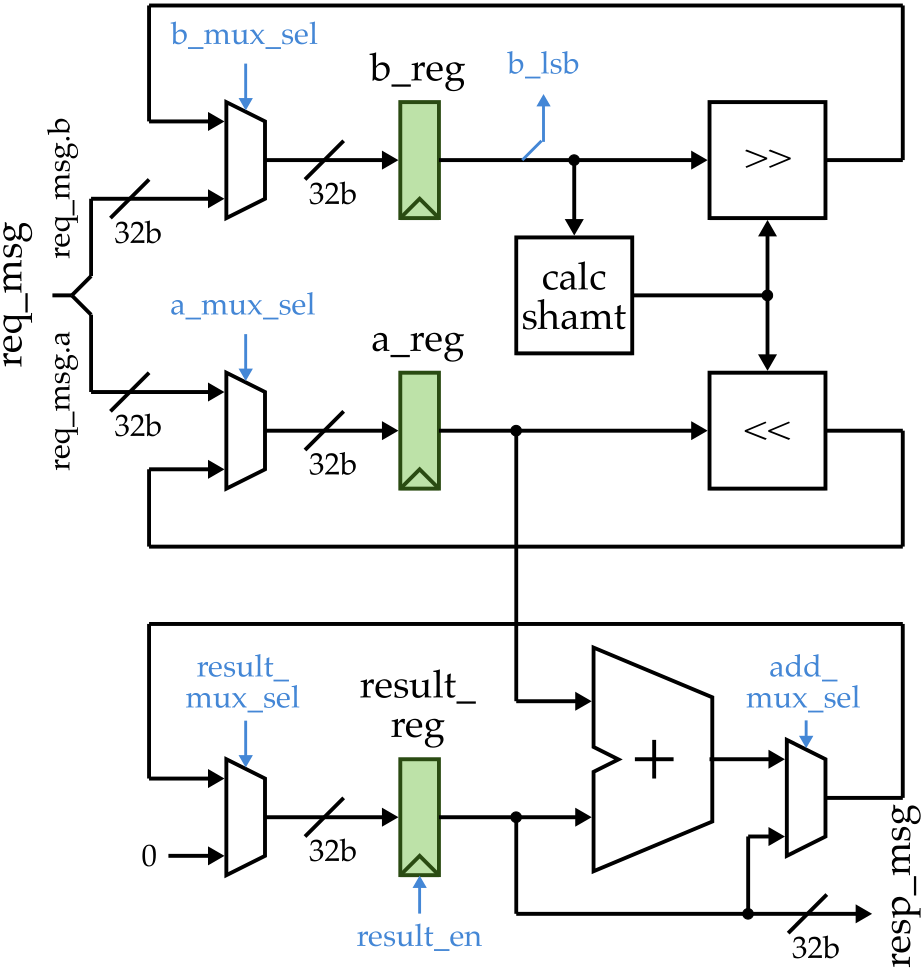
\includegraphics[width=0.5\textwidth]{images/20.png}
    \caption{Datapath for Variable-Latency Iterative Integer Multiplier – All datapath components are 32-bits wide except for the shift amount signal to the variable shifters.}
    \label{F20}
\end{figure}
\begin{figure}[H]
    \centering
    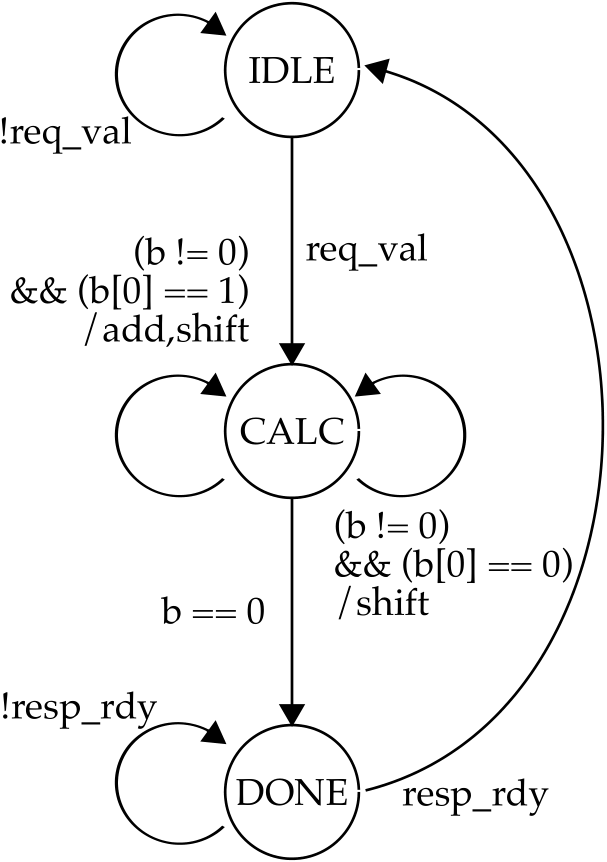
\includegraphics[width=0.45\textwidth]{images/21.png}
    \caption{Control FSM for Variable-Latency Iterative Integer Multiplier – Hybrid Moore/Mealy FSM with Mealy transitions in the CALC state.}
    \label{F21}
\end{figure}
While the iterative multipliers will likely require minimal area, they also require many cycles to calculate each result. As a point of comparison, we will also consider a simple single-cycle integer multiplier. Figure \ref{F22} shows the single-cycle RTL model. We use registered inputs for both the operands and the valid bit. If the response interface is not ready, then we stall the multiplier by disabling the register enable signals and combinationally propagating the response-ready signal to the request-ready signal. For the actual multiplier, we simply use the * operator; we will rely on the ASIC toolflow to choose the most appropriate multiplication hardware. The PyMTL and Verilog code for the single-cycle multiplier RTL model is in IntMulScyclePRTL.py and IntMulScycleVRTL.v, respectively.
\begin{figure}[H]
    \centering
    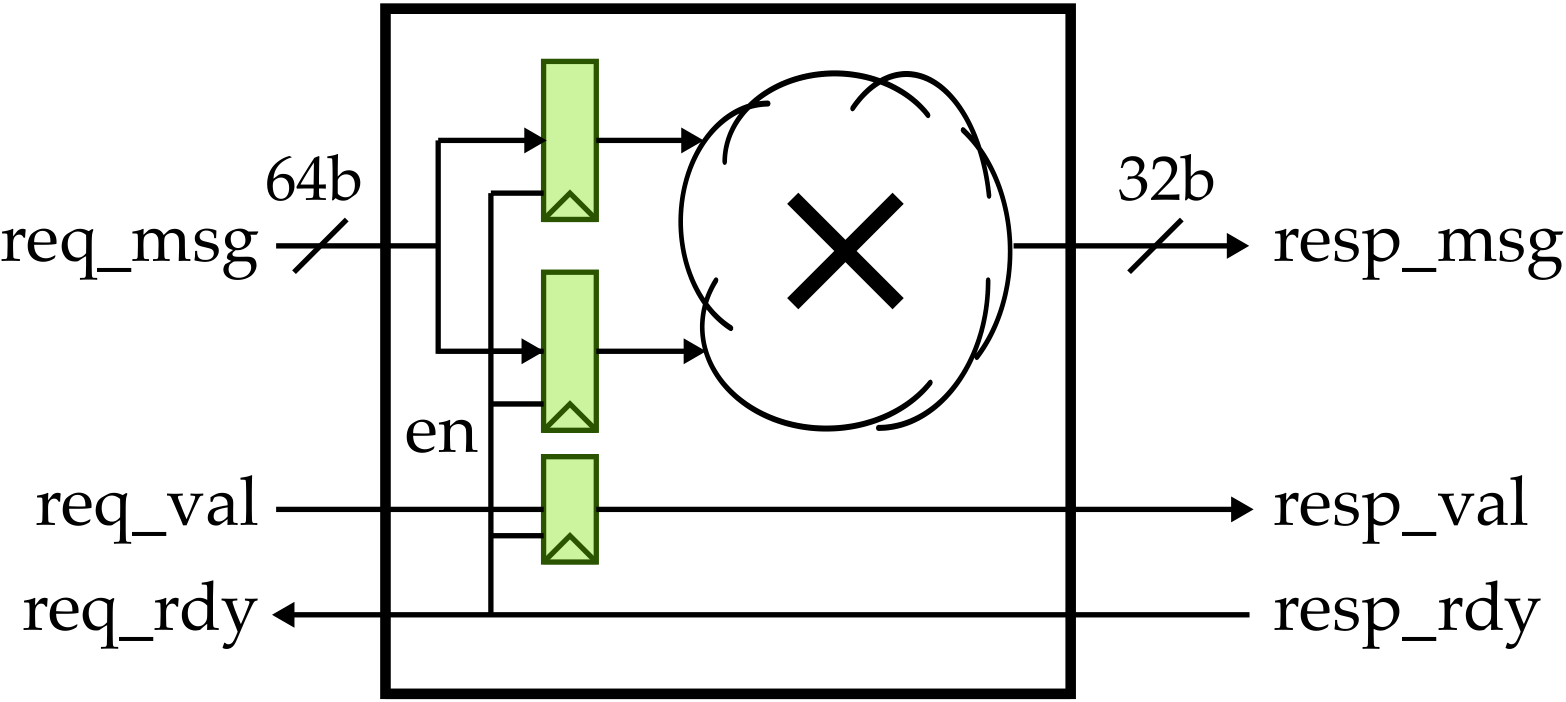
\includegraphics[width=0.6\textwidth]{images/22.png}
    \caption{Single-Cycle Integer Multiplier – We use registered inputs and combintionally connect the response ready signal to the request ready and the input register enable signals.}
    \label{F22}
\end{figure}
\subsubsection{Project Design}
For your alternative design, you should implement a pipelined integer multiplier with the same interfaces used in the baseline designs. You should implement an RTL model that is parameterized by the number of pipeline stages; you can assume that the number of stages will be either 1, 2, 4, or 8, although you can also support 16 and 32 stages if you like. As discussed in the labs, in this project, we will adopt the general policy of using registered inputs for larger blocks, so your pipelined multiplier should start with a set of pipeline registers.

The pipelined integer multiplier RTL model should use a child model that implements a single “partial product step” of the fixed-latency iterative multiplication algorithm. Each partial product step would involve three inputs: one for a, b, and result and three outputs also for a, b, and result. Each partial product step will perform two shifts, an addition, and then mux the result of the addition conditionally based on the least-significant bit of the b input. As always, you should unit test the partial product step model and potentially even build a composition of a few steps for integration testing. Once you are confident in your step model, implement the parameterized RTL model by using elaboration to insert the pipeline registers between the steps. Your pipelined multiplier should always include a total of 32 steps. What changes is just where you put the pipeline registers. If done correctly, your pipelined multiplier should be able to sustain one multiply transaction per cycle.

Note that there are many optimizations you might want to try that may lead to higher-quality hardware; you should feel free to explore different approaches if you like. For example, you might want to consider exploring the difference between using structural components within each partial product step vs. doing a flat design without any additional hierarchy within each partial product step. Or you may want to consider exploring the difference between an inelastic vs. elastic pipeline. In an inelastic pipeline, the entire pipeline stalls if the response interface is not ready. In an elastic pipeline, the pipeline can continue flowing even if the response is not ready as long as there are “bubbles” in the pipeline that can be eliminated. Or, possibly adding a queue at the response interface can enable better decoupling. Note if students want to explore more complicated multiplier microarchitecture, they should first implement a multiplier using a sequence of partial product steps. Once this first alternative design is working and evaluated, then students can implement another, more complicated alternative design in a different file with different tests.
\subsubsection{Testing Strategy}
We have provided you with all of the unit tests for the integer multipliers, although you will need to add your own test scripts for any new models you create. You are required to add more tests for your alternative design if you would like. Most of the unit tests are defined in \texttt{test/IntMulFL\_test.py}; the other test scripts reuse these unit tests as much as possible. You need a test that verifies your pipelined N-stage multiplier is, in fact, pipelining the multiplications with a cycle-accurate test. Note you may have to create new testing modules to validate the cycle accuracy within a test.
\subsubsection{Evaluation}
Once you have verified the functionality of your alternative design, you should then use the provided simulator to evaluate the cycle-level performance of the various multiplier designs. You can run the simulator for the first baseline design like this:
\begin{minted}{bash}
imul-sim --impl rtl-fixed --input small --stats
\end{minted}
The simulator will display the total number of cycles to execute the specified input dataset. You should study the line traces (with the \texttt{--trace} option) and the waveforms (with the \texttt{--dump-vcd} option) to understand the reason why each design performs as it does on the various patterns. For your pipelined multiplier, you can use the \texttt{--nstages} option to set the number of pipeline stages. Be careful to factor out the pipeline startup overhead for your pipelined multipliers for a fair comparison.

Once you have explored the cycle-level performance of the various multiplier designs, you should push the RTL models through the standard-cell ASIC toolflow to quantify the area, energy, and timing of each design. You need to push the following designs through the flow:
\begin{itemize}
    \item Fixed-latency iterative multiplier
    \item Variable-latency iterative multiplier
    \item Single-cycle multiplier
    \item Pipelined multiplier with one stage
    \item Pipelined multiplier with two stages
    \item Pipelined multiplier with four stages
    \item Pipelined multiplier with eight stages
\end{itemize}
For each design, you need to analyze the power/energy when executing three specific input datasets: small (small random numbers), large (large random numbers), and sparse (higher probability of zero bits in the input operands). You can generate the Verilog and VCD files for the fixed latency multiplier using the simulator like this:
\begin{minted}{bash}
imul-sim --impl rtl-fixed --input small --translate --dump-vtb
imul-sim --impl rtl-fixed --input large --translate --dump-vtb
imul-sim --impl rtl-fixed --input sparse --translate --dump-vtb
\end{minted}
You can optionally use \texttt{mflowgen} to accelerate your ASIC flow. You can choose to use the Verilog model or the PyMTL3 model.

For the baseline iterative designs, you can set the clock constraint to 0.6 ns, and for the baseline single-cycle design, you can set the clock constraint to 1.5 ns. For your pipelined multiplier, you will need to experiment to find a good clock constraint. If you have no negative slack, you are not pushing the tools hard enough. If you have too much negative slack, you are pushing the tools too hard. Remember that every design must meet timing after place and route!

Be sure to look at the reports from each run to analyze your results, especially the timing and area reports. Also, confirm that your results seem reasonable in case part of the design was aborted by the standard-cell ASIC flow since it can be difficult to see when using the automated scripts. In addition to tables and bar plots, you should include several "energy vs. performance" plots to compare the various designs. We recommend having one energy vs. performance plot per input dataset, so plot the results for all of the different microarchitectures executing this dataset on one plot and then create another plot for a different input dataset. These "energy vs. performance" plots should enable you to provide deep insight into the various trade-offs in the evaluation section of your report. If you also implemented a more complicated multiplier microarchitecture, then you must evaluate it in the alternative design section.
\subsubsection{Tasks}
\begin{itemize}
    \item Complete TODO and PROJECT TASKS sections.
    \item Project Design Section – In the project design section of your report, you should briefly discuss how you created a parameterized pipelined multiplier. Be sure to include a diagram illustrating your design. If you also implemented a more complicated multiplier microarchitecture, then you must describe it in the project design section.
    \item Evaluation Section
\end{itemize}

\subsection{Open-ended Project I}
Propose a project that falls in the scope of SoC design and evaluate it using any flows that are available to you. You are free to combine it with ongoing research from your own studies or with another course, provided the scope of the project implementation submitted for this course is sufficient. 

\subsection{Open-ended Project II}
Propose a plan to reproduce (part of) the main design of existing research work. You can reproduce any design (after approval) in the last 15 years of Top SoC conferences (SOCC, ISCA, MICRO, HPCA, ISSCC, JSSC, etc.) publication. You can choose any proper flow to reproduce it. You need to decide how to verify/evaluate it.

\subsection{Open-ended Project III}
For those who are interested in hardware accelerator of machine learning, implement a certain type of neural network like a convolutional neural network, a support vector machine, or other machine learning algorithms like k-means or LSTM by HLS or HDL or MATLAB HDL Coder/Simulink, optimize the design by parallelism, package an IP core, do synthesis and implementation, and analyze and evaluate by Vitis or Pynq on the FPGA board. The general requirements are the same as other topics. You can learn from Xilinx Research Labs' FINN experimental framework for deep (quantized) neural network inference on FPGAs \cite{finn}.

\newpage

\section{Deliverable}
\begin{itemize}
    \item Group Deliverable:
    \begin{itemize}
        \item A well-presented project report that has a clear problem definition, your implementation details, any novelty, your evaluation methodology, detailed simulation results and evaluation results, and future work. No format requirement, but \href{https://www.ieee.org/conferences/publishing/templates.html}{IEEE proceeding format} is highly preferred.
        \item Pack your implementation code, test benches, and other necessary files into one zip file. Please also include a copy of the Tcl script that you have used for running the flow.
        \item Project demo \& presentation – A project presentation session will be held. A 3-min demo session + 10-min presentation + 2-min questions for each group. Slides need to be uploaded as part of the deliverable. Each student needs to present their part. All need to participate in the presentation session.
    \end{itemize}
    \item Individual Deliverable
    \begin{itemize}
        \item Complete the peer-evaluation form appended at the end of this document.
    \end{itemize}
\end{itemize}


\section{Honor Code Policy}
If you reuse others' codes, you must add proper citations and references and include the licenses if there are any; otherwise, it is a violation of the Honor Code.

\section{Timeline}
This is a 4-week project assignment; the intent is to allow you to plan and execute a significant, open-ended design exploration and mapping. You will not achieve the implementation goal or the course learning goals by trying to do this in one week. We give you a timeline to help provide some structure, but the milestones are minimal, and doing the minimum to hit the milestone each week will be insufficient to get you where you need to be at the end. We are giving you flexibility in planning and ordering rather than lock-step specifying exactly what you need to do each week. Also, please note that a group/team project is a great experience for exercising your ability to collaborate with peers. Thus, everyone needs to contribute to make the project a success. Please watch out for the following major timelines.

\begin{itemize}
    \item By 23:59 November 16th (Wednesday), please indicate your preferred project topic by filling \href{https://wenjuan.feishu.cn/m?t=sKyT2NHNiuHi-nwym}{this survey}. Eventually, each team will work on a unique topic. To make the selection, each team needs to rank the top 5 preferences. We will try to accommodate based on your preferences and the time stamp when you submit your decision, but please note that top 1 preferences might not be guaranteed. Please also note that all projects are designed equally in terms of the amount of work and effort to spend, so if you are not able to select your top choice, it is totally ok. To reduce the interruption to the actual project execution, you won’t be able to change your topic after the selection deadline unless being approved by the instructor/TA. The selection results will be annouced on 17th.
    \item Around December 1st (Thursday), milestone check sessions will be scheduled to check the progress of each team. Each team will need to report their current progress and difficulties briefly. Failure to do so will result in your project being marked as incomplete.
    \item On December 8th, during the last lecture (14:00-15:40), your group must do a final presentation. Your presentation should be $\sim$13-minute long (together with a small demo), $\sim$15-minute in total, including questions. Everybody in your group must present; your individual grade will include your presentation. Since you will present before your final report is due, you will not be expected to present a complete, fully functional project. Good presentations (and write-ups, for that matter) will cover the specific sub-projects you chose to implement and how you implement it. Very detailed descriptions of your project are not appropriate for a 13-minute presentation. The presentation will be graded by the teaching group based on the quality of the results and the ability to answer all the questions (including clarification questions).
    \item By 23:59 December 14th, please submit your complete report and final slides along with the code and scripts.
\end{itemize}


\section{Grading Policy}
\begin{itemize}
    \item Milestone check 10\%
    \item Presentation \& slides 20\%
    \item Report \& documentation 15\%
\end{itemize}
\begin{itemize}
    \item Implementation of base features 15\%
    \item Correctness and testing 15\%
    \item Performance optimization 10\%
    \item Analysis 15\%
    \item Additional features (upto 15\%: Extra points for those who attempt with ambitious designs.)
    \item For excellent implementations, your work will be proposed to publish your results at top conferences/journals. The instructor/TA will help throughout the process.
\end{itemize}

\section{Recommendations}
\begin{itemize}
    \item Pick the application based your \textbf{interests} instead of ``easiness''. You will need to take the ownership of your topic once you make the selection.
    \item Start as soon as possible, and plan carefully. 
    \item All team members need to contribute. This is very important to make the project a success.
    \item Ask question immediately if you get stuck.
\end{itemize}

\newpage
\appendix
\section{Peer Evaluation Form}
\begin{table}[H]
    \centering
    \begin{tabular}{|c|c|c|c|c|}
        \hline
        Part & Your work & Your partner's work & Your score & Your partner's score \\
        \hline
        & & & & \\
        \hline
        & & & & \\
        \hline
    \end{tabular}
\end{table}

\section{General Report Guidelines}
\begin{itemize}
    \item Abstract: Summarize the main contribution(s), and list any key findings.
    \item Introduction: Describe the problem your work addresses, why it is important, and overview the solution (if you are proposing one).
    \item Related Work: Overview of the relationship of your work to prior work, with citations. It’s of course okay if the work is not 100\% novel.
    \item Methods: Detail the proposed design or methods (this may span one or more sections). This includes the design of any algorithms, hardware structures, interface strategies, codesign techniques, etc. Be sure to use drawings/figures/code-examples that can help explain the ideas.
    \item Methodology: Describe your approach for how you evaluated the work, and explain why it is fair or valid.
    \item Evaluation: Provide and analyze any quantitative results.
    \item Conclusions: Summarize the findings and main contributions, as well as any ideas for future work.
    \item Statement of Work: For each student in the group, describe the tasks that they performed.
    \item References: List all references cited.
\end{itemize}

\section{General Presentation Guidelines}
In this short presentation, you should motivate your audience (start with some background to connect with what we have learned), and highlight the contributions of your project. You can even choose to interact with your audiences and prepare questions for discussions. There are no limitations on the template to use or how many slides you need to have. The rule of thumb is usually one minute per slide. The following are several links and tips you might find helpful.
\begin{itemize}
    \item Top 5 Tips to a Successful Conference Presentation \url{https://mitendicotthouse.org/top-5-tips-to-a-successful-conference-presentation/}
    \item How to give a technical presentation (how to give a scientific talk) \url{https://homes.cs.washington.edu/~mernst/advice/giving-talk.html}
    \item Guidelines for Oral Presentations \url{https://ocw.mit.edu/courses/biological-engineering/20-109-laboratory-fundamentals-in-biological-engineering-spring-2010/assignments/guidelines-for-oral-presentations/}
\end{itemize}

 A few tips for a good presentation:
\begin{itemize}
    \item Well-defined scope
    \item Well-balanced text vs. pictures
    \item Pick up only one aspect, clearly describe the novelty of the work
    \item Always think from your audiences’ perspectives; in this case, your audiences will be your peers
    \item Proper references are required
    \item Good time management
    \item Being confident
    \item Eye contact is important
\end{itemize}

\section{Change Log}
\subsection{Fall 2022}
Prof. Xinfei Guo and Yihua Liu
\begin{itemize}
    \item Word to LaTeX
    \item Delete 2 topics and add 11 new topics
    \item Add the flow descriptions and diagrams
\end{itemize}
\subsection{Fall 2021}
Prof. Xinfei Guo
\begin{itemize}
    \item Create the project topics
\end{itemize}

\printbibliography
\end{document}
